\documentclass[11pt]{article}

\usepackage[utf8]{inputenc}
\usepackage[T1]{fontenc}
\usepackage{geometry}
\usepackage{graphicx}
\usepackage{hyperref}
\usepackage{float}
\usepackage{caption}
\usepackage{subcaption}
\usepackage{enumitem}
\usepackage{xcolor}
\usepackage{amsmath}

\geometry{margin=1in}

\title{Pokémon ML Predictor}
\author{}
\date{}

\begin{document}

\maketitle

This project aims to predict the \texttt{BST}, known as \texttt{total\_stats} (sum of base stats: HP + atk + def + sp.atk + sp.def + spe) for existing and future Pokémon generations using a scraped dataset of all 1025+ Pokémon including regional forms.

The prediction will be achieved by using \textbf{Machine Learning} and \textbf{Feature Engineering}.

\tableofcontents
\newpage

\section{Feature's Description (Our initial Pokedex*)}

\textit{(The pokedex is the animal atlas of the pokemon world. It collects information of all known species)}

Every Pokémon can be categorised based on its basic attributes:

\begin{itemize}
    \item \texttt{BST}: base stat points. In general terms, it describes how ``strong'' a Pokémon is. It ranges from 175 to 720.
    \item \texttt{type(s)}: like \texttt{Electric} (i.e. Pikachu), \texttt{Fire}/\texttt{Flying} (i.e. Charizard), etc. Total 18 different ones as unique or pairs of.
    \item \texttt{height}: 0.1 to 20 m.
    \item \texttt{weight}: 0.1 to 999.9 kg.
    \item \texttt{color}: The main color of the Pokémon. See \href{https://bulbapedia.bulbagarden.net/wiki/List_of_Pok%C3%A9mon_by_shape}{this link} for more information.
    \item \texttt{shape}: There are 14 different shapes (\texttt{upright}, \texttt{quadruped}, etc.). See \href{https://bulbapedia.bulbagarden.net/wiki/List_of_Pok%C3%A9mon_by_color}{this link} for more information.
    \item \texttt{stage}: Pokémon can evolve. A Pokémon cannot evolve more than 2 times. See next section for further information.
    \item \texttt{category}: Majority of Pokémon belong to the \texttt{regular} category. There are \texttt{legendary} ones like Articuno, Moltres, Mewtwo, and \texttt{mythical} ones, like Mew.
\end{itemize}

Game Freak, the Pokémon Company, usually provide the first three ones when a new Pokémon is announced. For example, see these three \href{https://windswaves.pokemon.com/en-us/}{new Pokémon} for the new games to come in 2027. The rest of the features (\texttt{color}, \texttt{shape}, \texttt{stage}, and \texttt{category}) are easily extracted from visuals and little experience within the franchise.

\texttt{Stage} requires more experience with the franchise (i.e. one would never expect a Charizard to be the first stage of an evolution chain of two stages!, but other Pokémon, like \href{https://bulbapedia.bulbagarden.net/wiki/Archaludon_(Pok%C3%A9mon)}{Archaludon}, could be hard to determine at sight).

The next section will be devoted to extracting information from all these features. In this way, we will get further insights on how each are related to each other and which ones can be combined to create secondary features through feature engineering.

\section{Data Analysis}

\subsection{BST Distribution Across Generations}

Pokémon is an old franchise which started in 1996. Therefore, not all 1082 different species were ``discovered'' by years. With each new generation of games, new Pokémon are included, increasing the quantity of these creatures. We can then first explore how these \texttt{BST} values have changed since 1996.

\begin{figure}[H]
    \centering
    \begin{subfigure}{0.47\textwidth}
        \centering
        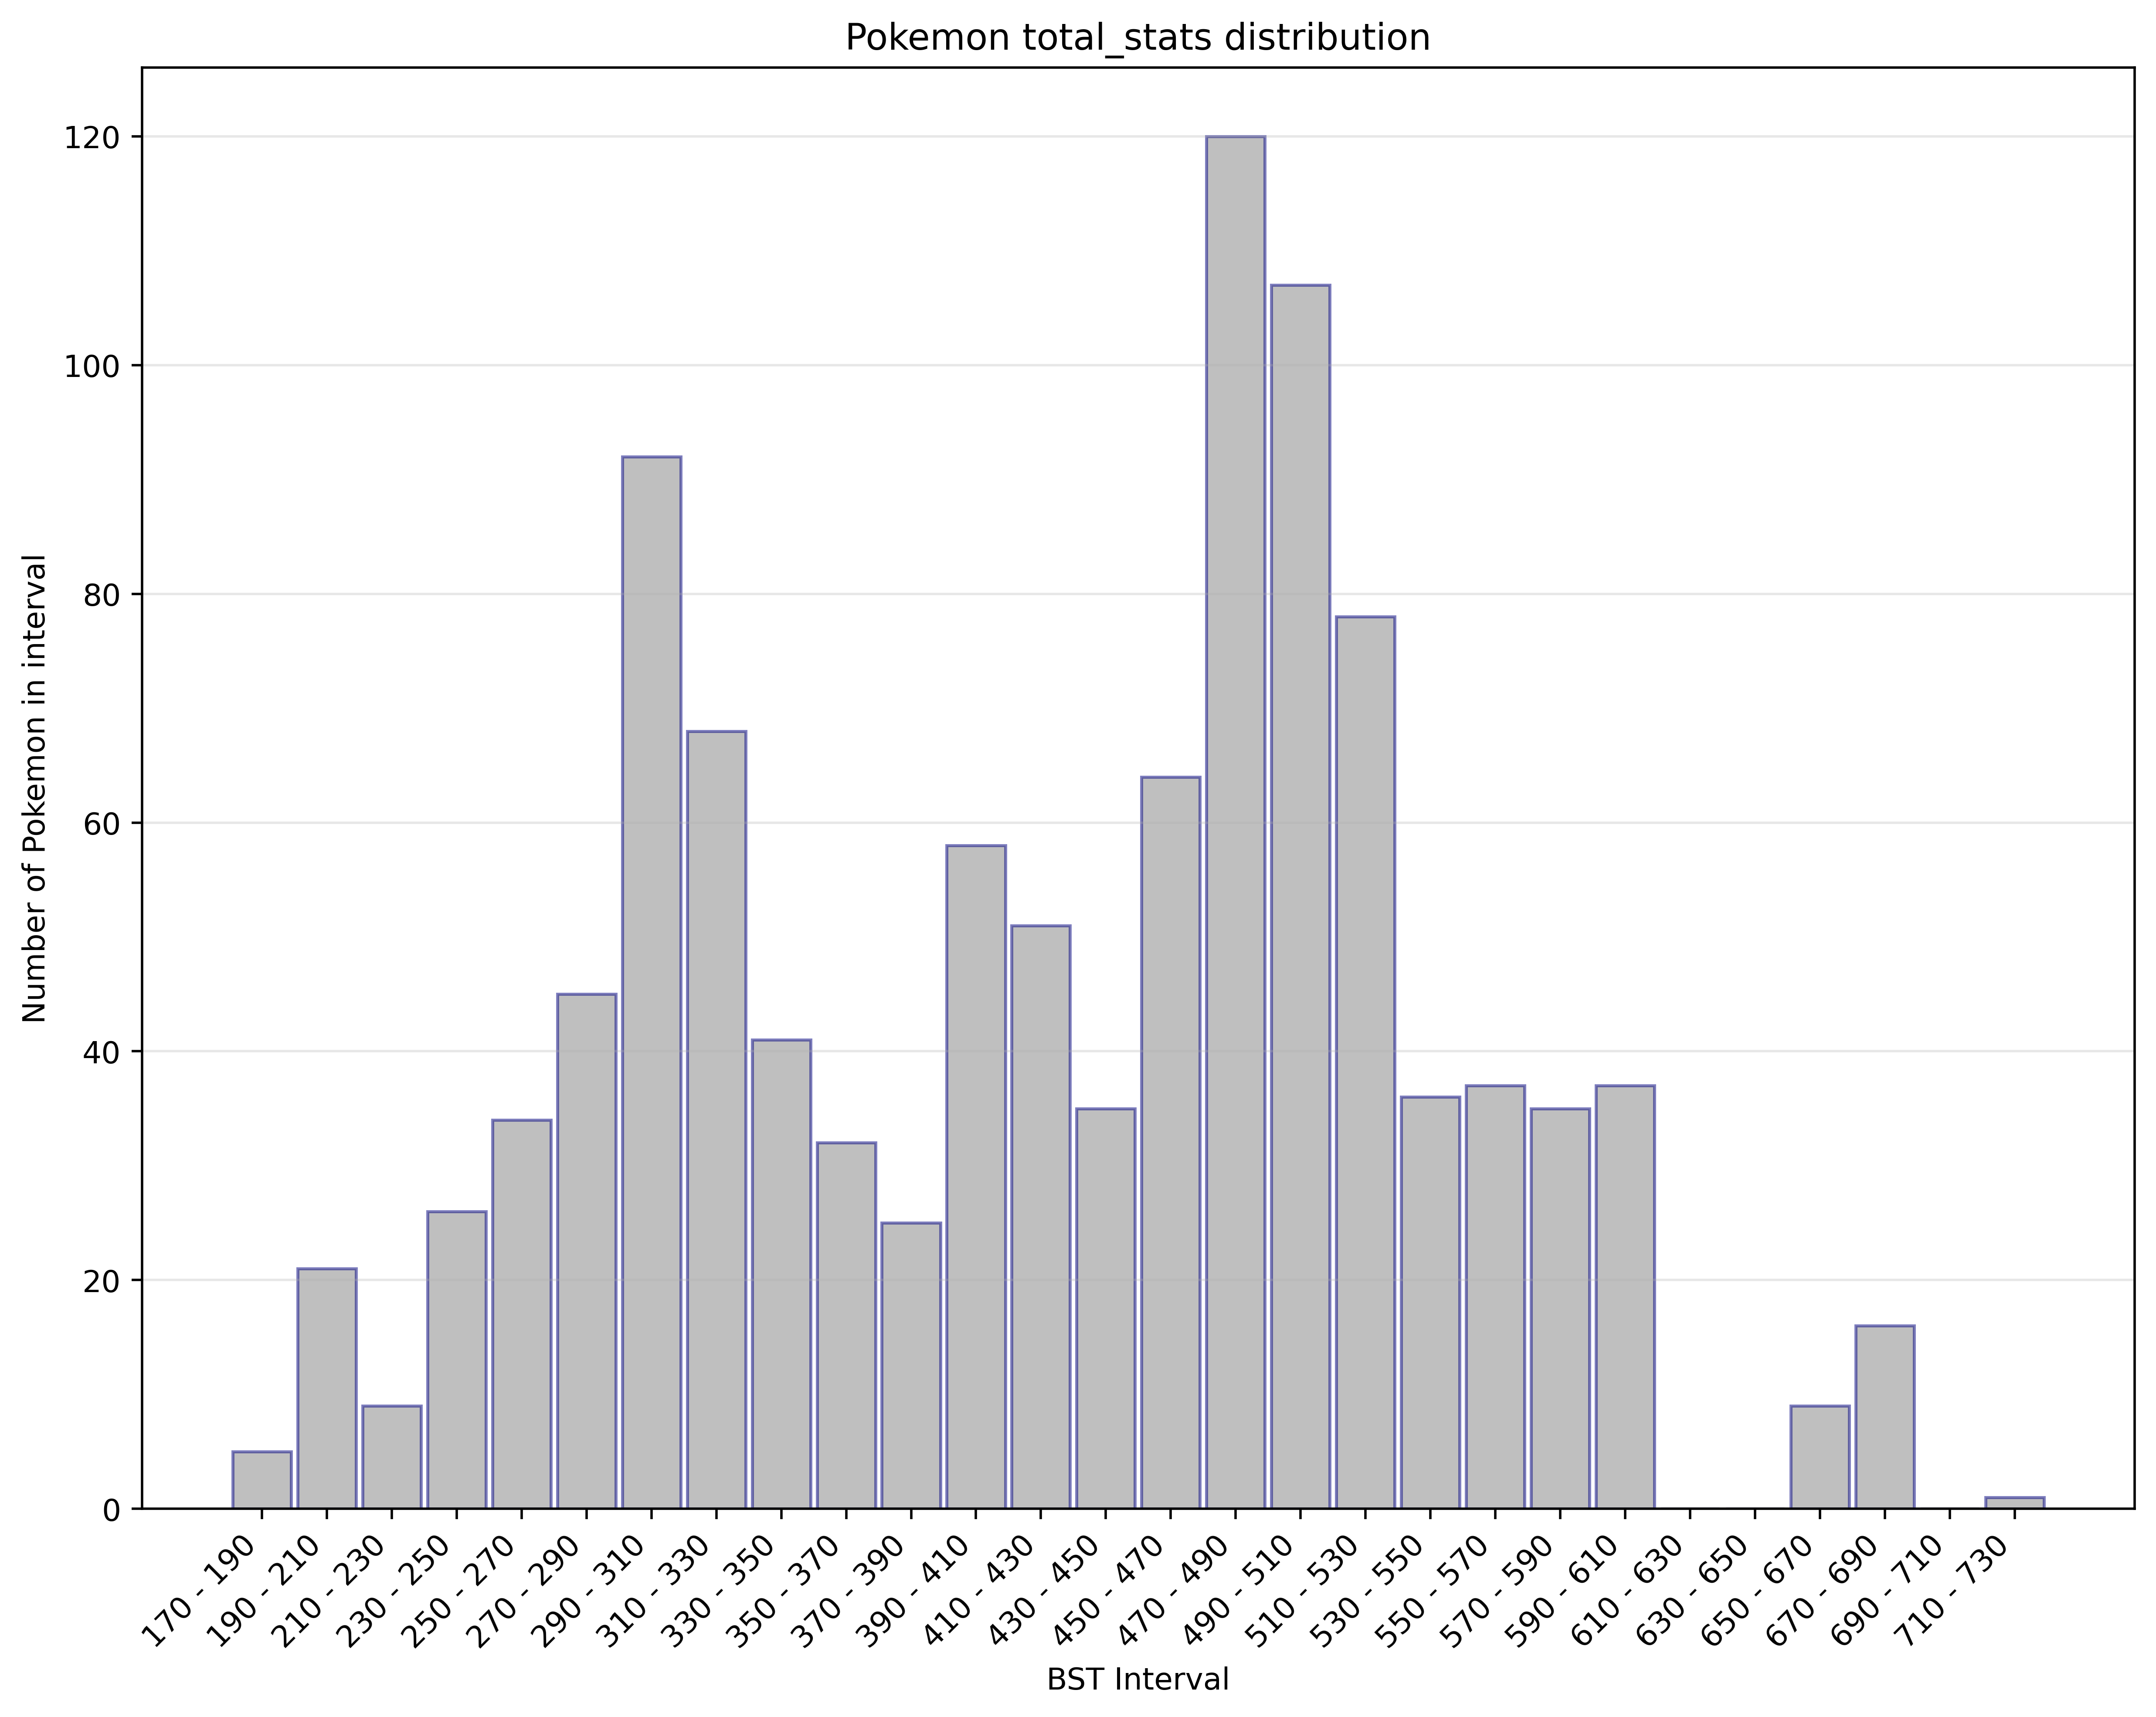
\includegraphics[width=\linewidth]{../plots/total_stats_interval.png}
        \caption{BST interval distribution}
    \end{subfigure}
    \hfill
    \begin{subfigure}{0.47\textwidth}
        \centering
        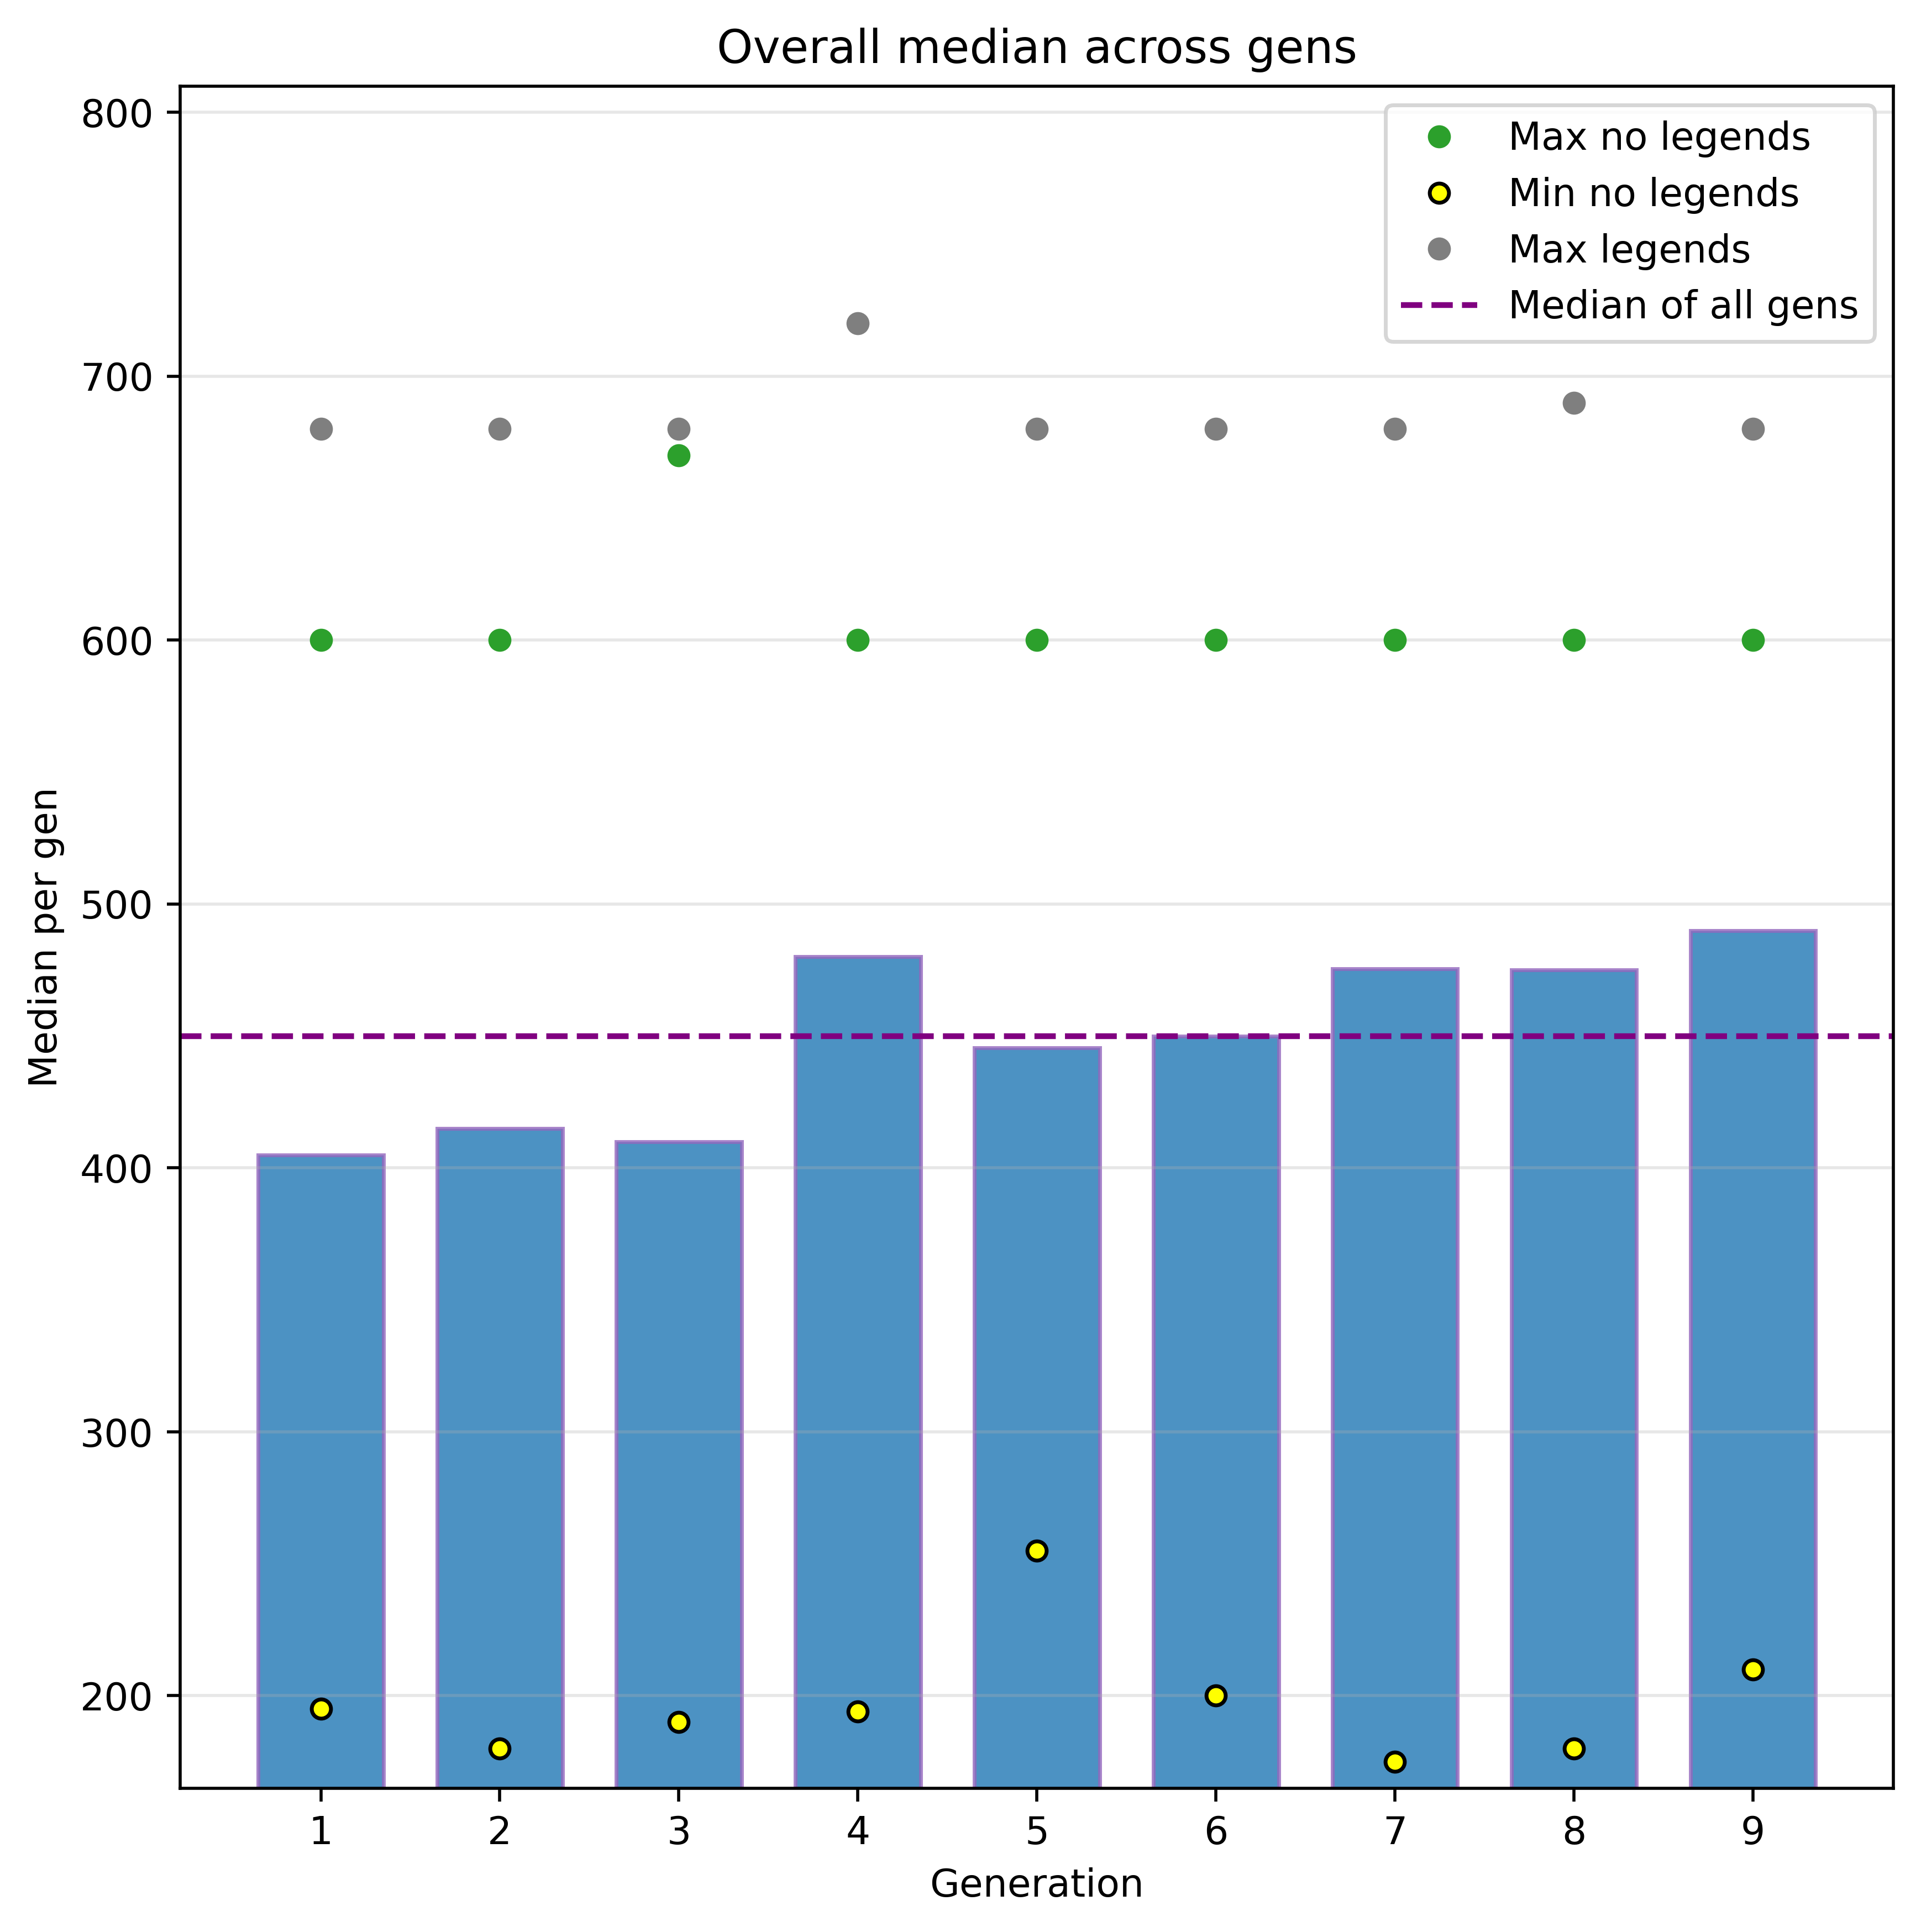
\includegraphics[width=\linewidth]{../plots/median_dic.png}
        \caption{Median BST by generation}
    \end{subfigure}
\end{figure}

In the first plot we can see how Pokémon are distributed from the minimal value of \texttt{BST} to the maximum one in intervals of 20 units. In fact, we see that there are two main cluster intervals: (270--330) and (450--490). We will later see what these correspond to when comparing to the \texttt{stage} in the evolution chain.

The second plot shows the median of \texttt{BST} for each generation that has been released in the last 30 years. This median seems to agree with the second cluster of \texttt{BST} in the first image. Overall, we can see that the median has been increasing over generations. This may point to the fact that there exists some power-creep (i.e. Pokémon are getting stronger and stronger designs in each generation) that could be useful to account for when training the model.

The second plot also displays the minimum and maximum value of \texttt{BST} for each generation (corresponding to one or more Pokémon in that generation). We can also see the overall median across all generation. It is also worth noting the behaviour of min/max values for each generation.

\begin{itemize}
    \item The minimum value seems to be under or equal to 200 points, with generations 5 and 9 showing outliers.
    \item On the other hand, if we exclude \texttt{legendary} Pokémon, we see that the maximum value for \texttt{BST} of \texttt{non-legendary} Pokémon is quite constant across generation, except for generation 3*. This seems to impose an upper limit for any \texttt{non-legendary} Pokémon that has not been broken in a long time.
    \item For \texttt{legendary} Pokémon we see the value seems also to be limited above by 700 points. Only generation 4 crossed this barrier (Arceus, the ``God'' of all Pokémon, was introduced in this generation).
\end{itemize}

\paragraph{Summary BST across generation}
\begin{itemize}
    \item \texttt{BST} seems to cluster around (270--310) and (450--490).
    \item \texttt{BST} seems to increase a little each generation.
    \item \texttt{BST} max for \texttt{regular} Pokémon looks limited at 600.
\end{itemize}

\noindent
\textit{(* Game Freak designers were slaking off in that generation)}

\subsection{BST Distribution by Evolution Chain Stage and Category}

Let us now explore how the \texttt{BST} behaves for each evolution chain stage and category. First, it is important to explain how we are going to catalogue each stage.

\begin{itemize}
    \item \texttt{Babies2} $\rightarrow$ First stage of an evolution chain of 2 stages. (i.e. Ekans, Ratatta, etc.)
    \item \texttt{Babies3} $\rightarrow$ First stage of an evolution chain of 3 stages. (i.e. Charmander)
    \item \texttt{F2} $\rightarrow$ Second stage of an evolution chain of 2 stages. (i.e. Sandlash)
    \item \texttt{F3} $\rightarrow$ Third stage of an evolution chain of 3 stages. (i.e. Charizard)
    \item \texttt{Inter} $\rightarrow$ Second stage of an evolution chain of 3 stages. (i.e. Charmeleon)
    \item \texttt{Single} $\rightarrow$ No evolution chain. (i.e. Ditto)
\end{itemize}

\begin{figure}[H]
    \centering
    \begin{subfigure}{0.58\textwidth}
        \centering
        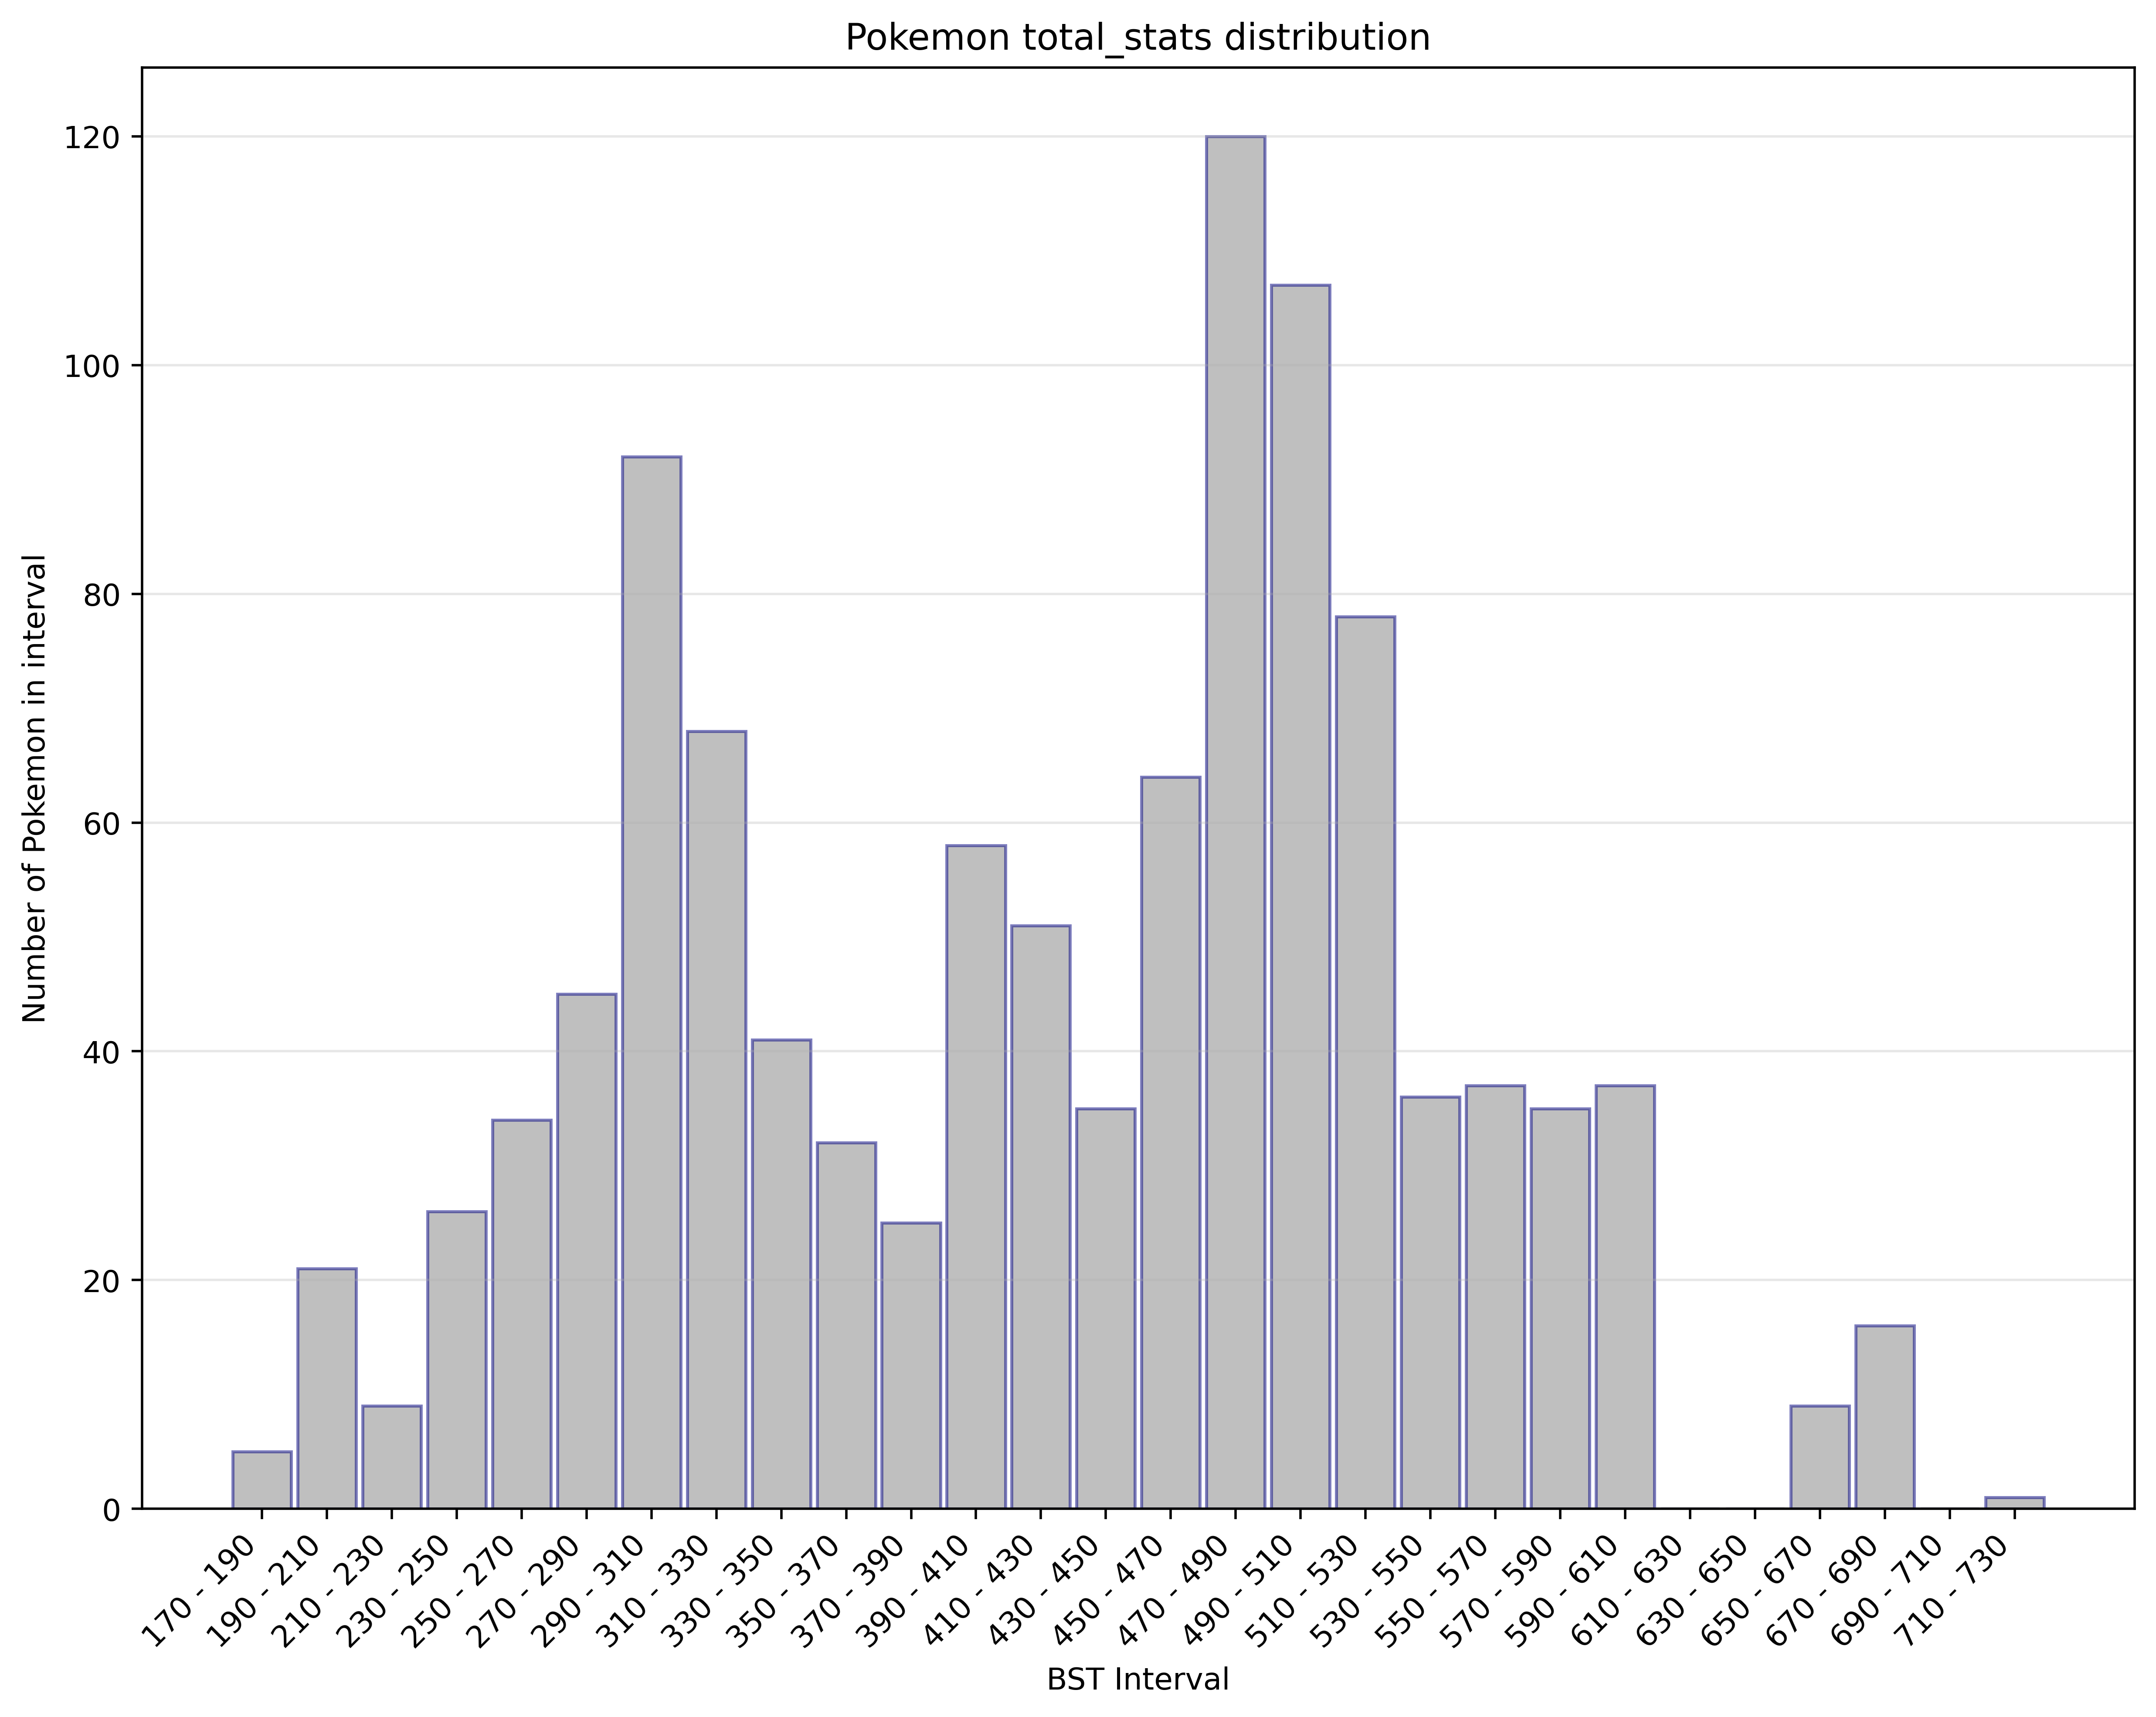
\includegraphics[width=\linewidth]{../plots/total_stats_interval.png}
        \caption{BST Intervals Distribution}
    \end{subfigure}
    \hfill
    \begin{subfigure}{0.38\textwidth}
        \centering
        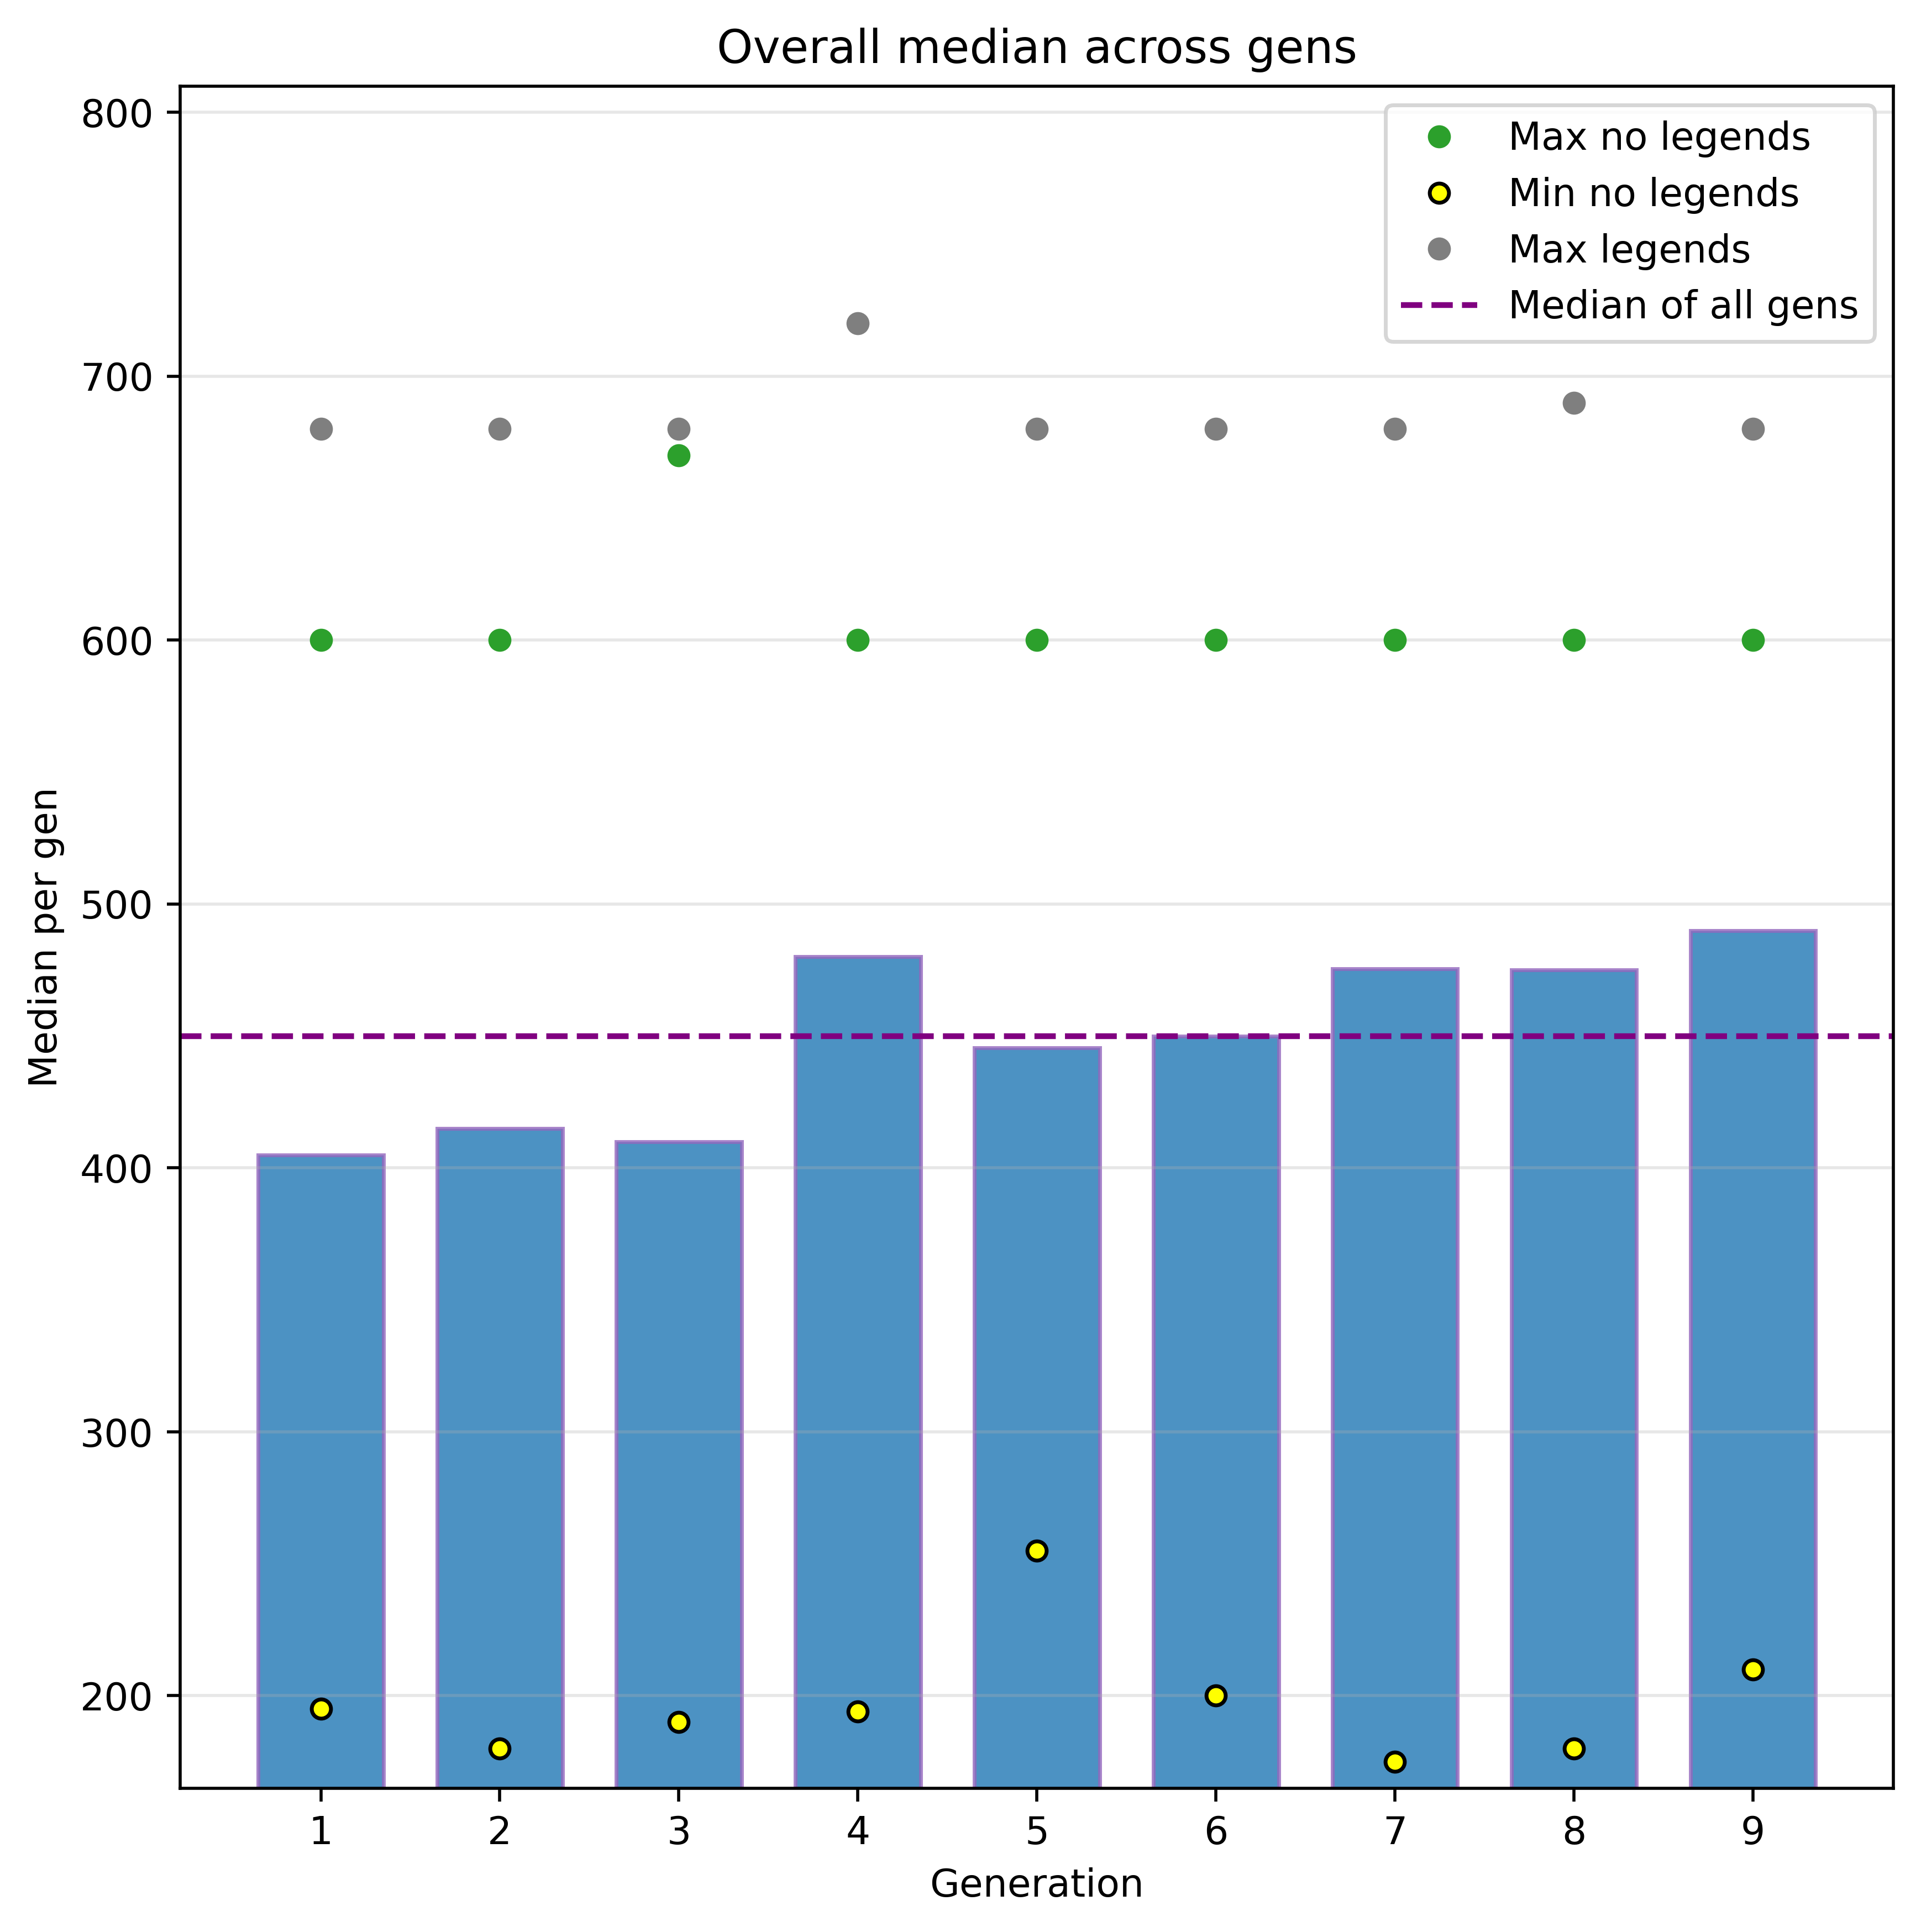
\includegraphics[width=\linewidth]{../plots/median_dic.png}
        \caption{Median Evolution by Generation}
    \end{subfigure}
\end{figure}

Here we can also extract juicy information:

\begin{itemize}
    \item \textbf{F3 (final stage, 3-stage chain):} This trend seems to follow a cubic polynomial around the median.
    \item \textbf{Babies (pre-evo):} No clear pattern regardless of chain length.
    \item \textbf{Singles:} While generations 1 and 2 had powerful single evolution Pokémon, it decreased in the two following ones and kept a steady growth from Gen 5.
    \item \textbf{Inter (stage 2 of 3):} This seems to nicely adjust to the overall median across generation. However, there is a slight favorability from Gen 7+.
    \item \textbf{Legendaries:} Gen 7 dip due to Cosmog line, which is a \texttt{legendary} Pokémon with an evolution chain of 3 stages.
\end{itemize}

In fact, it could be illuminating if we try to fit different polynomials to two clear patterns in F3 and Singles (from third generation onwards).

\subsubsection{F3 Mean/Median (cubic fit)}

\begin{figure}[H]
    \centering
    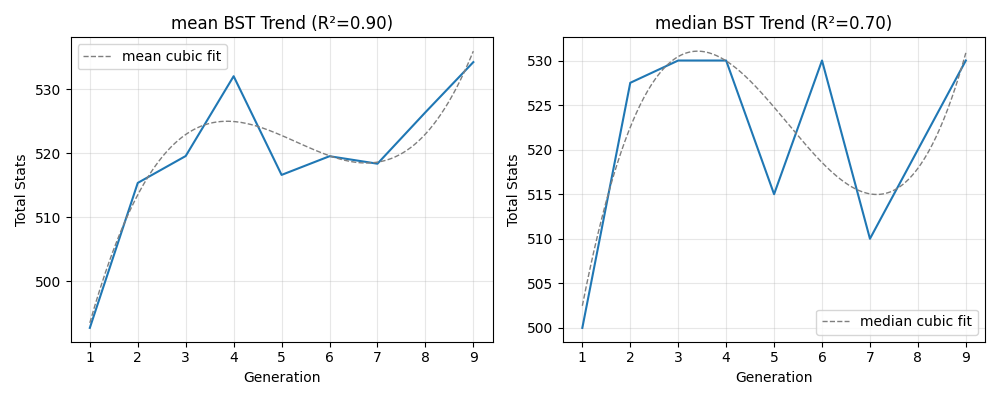
\includegraphics[width=0.8\textwidth]{../plots/bst_f3_fit.png}
    \caption{F3 polynomial fit}
\end{figure}

The \(R^2 > 0.7\) for the median indicates a strong ongoing trend. This can be useful for \textbf{feature engineering}.

\subsubsection{Singles Linear Fit (Gen 3+)}

\begin{figure}[H]
    \centering
    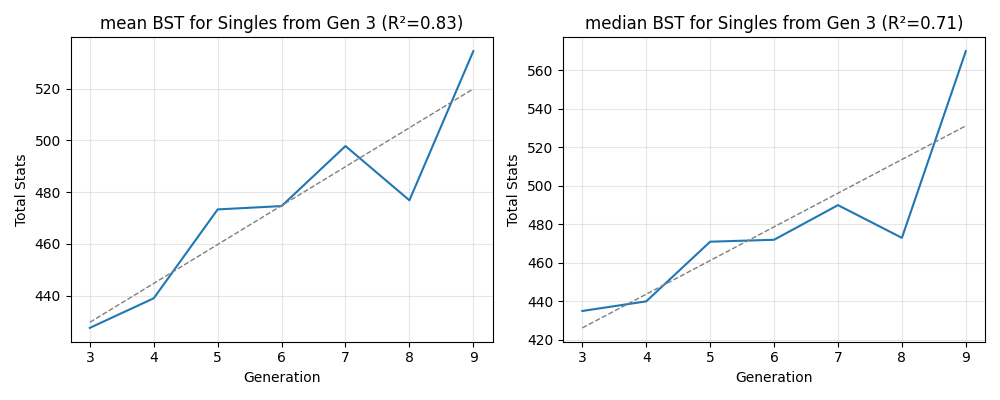
\includegraphics[width=0.8\textwidth]{../plots/bst_single_fit.png}
    \caption{Singles linear fit}
\end{figure}

As we suspected, the median trend for this stage is quite strong also, with \(R^2 \approx 0.7\). This can also be important to keep in mind when engineering new attributes.

\paragraph{Summary BST for stage and category}
\begin{itemize}
    \item \texttt{BST} for the final \texttt{stage} of an evolution chain of 3 has followed a clear cubic trend.
    \item \texttt{BST} for \texttt{single} stage has grown steadily since generation 3.
\end{itemize}

\section{Type Order Impact Analysis}

\subsection{Type Deviations from Stage Medians (Non-Legendaries)}

\begin{figure}[H]
    \centering
    \begin{subfigure}{0.32\textwidth}
        \centering
        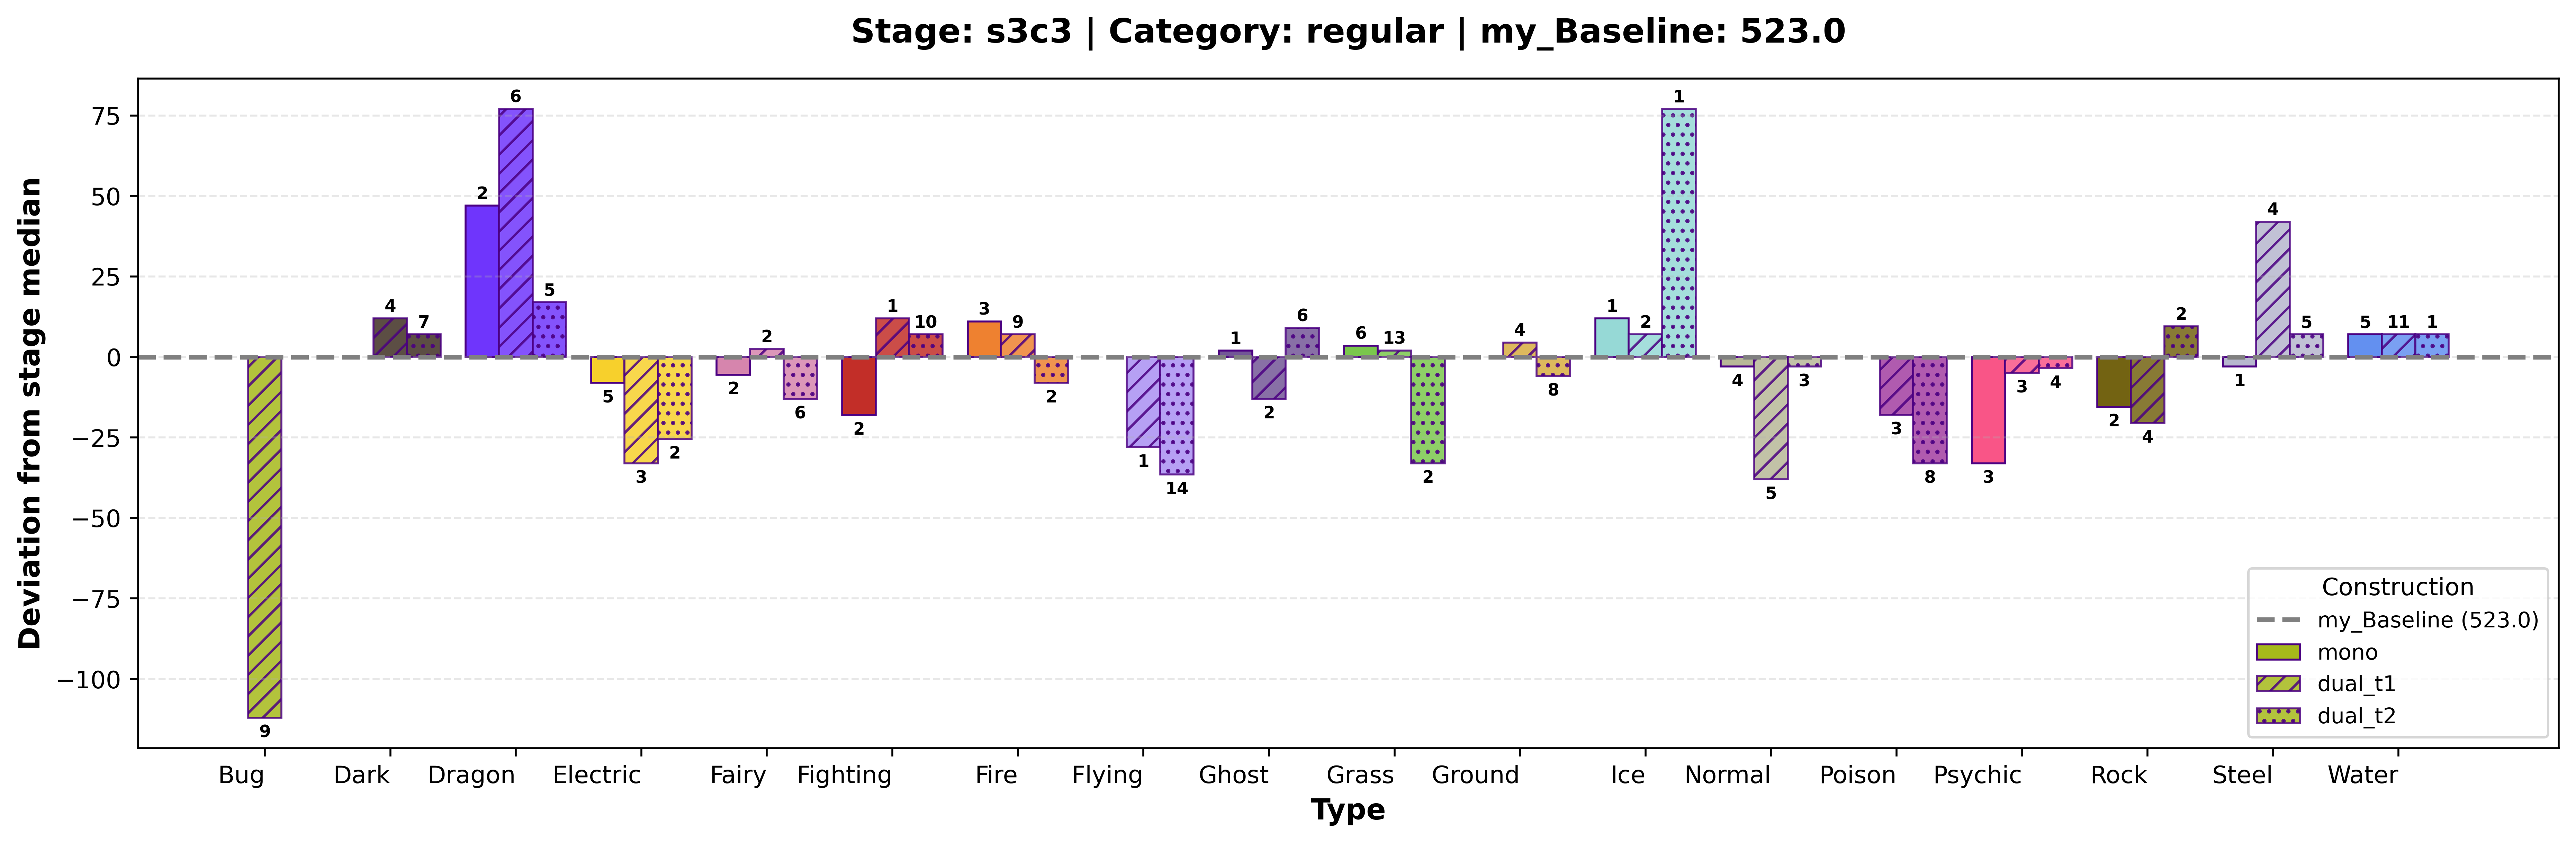
\includegraphics[width=\linewidth]{../plots/type_dev_s3c3.png}
        \caption{Type deviations S3C3}
    \end{subfigure}
    \hfill
    \begin{subfigure}{0.32\textwidth}
        \centering
        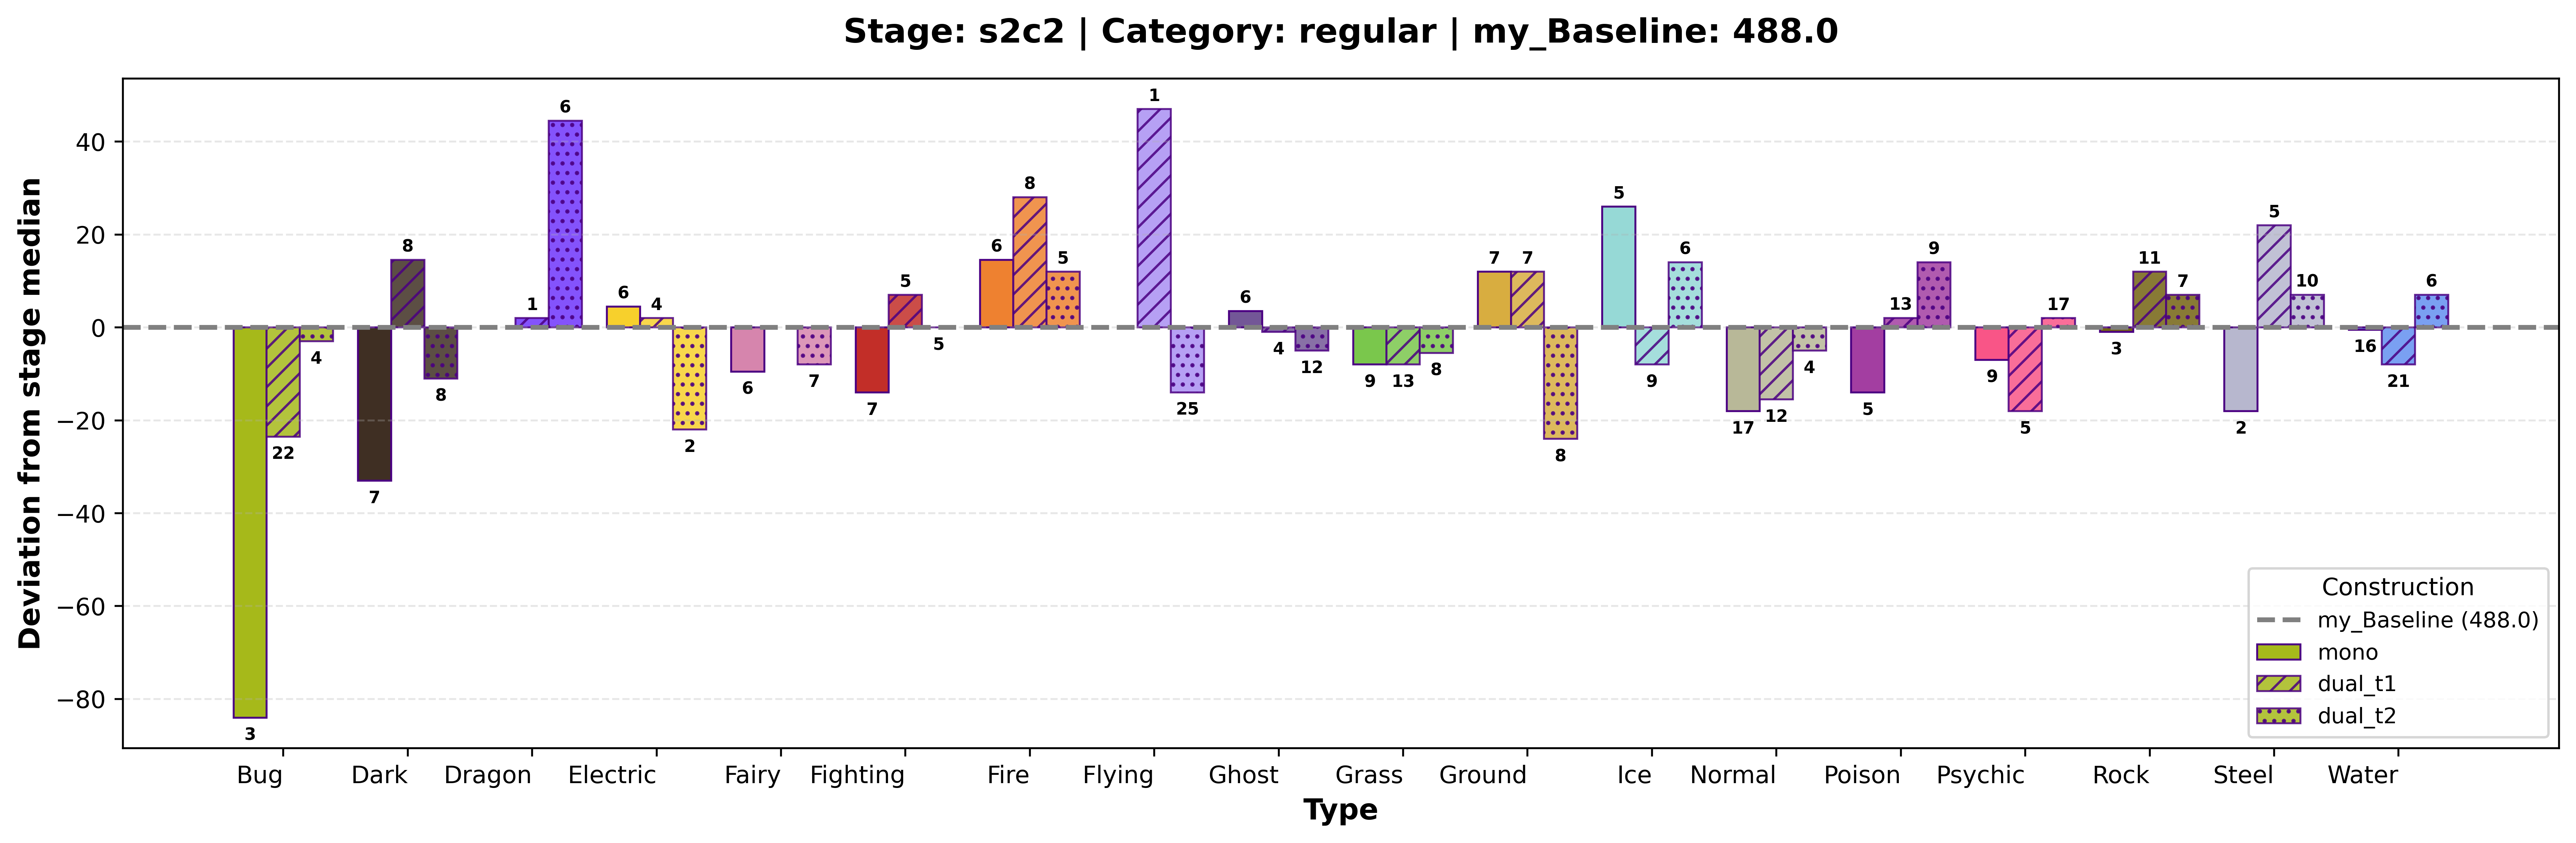
\includegraphics[width=\linewidth]{../plots/type_dev_s2c2.png}
        \caption{Type deviations S2C2}
    \end{subfigure}
    \hfill
    \begin{subfigure}{0.32\textwidth}
        \centering
        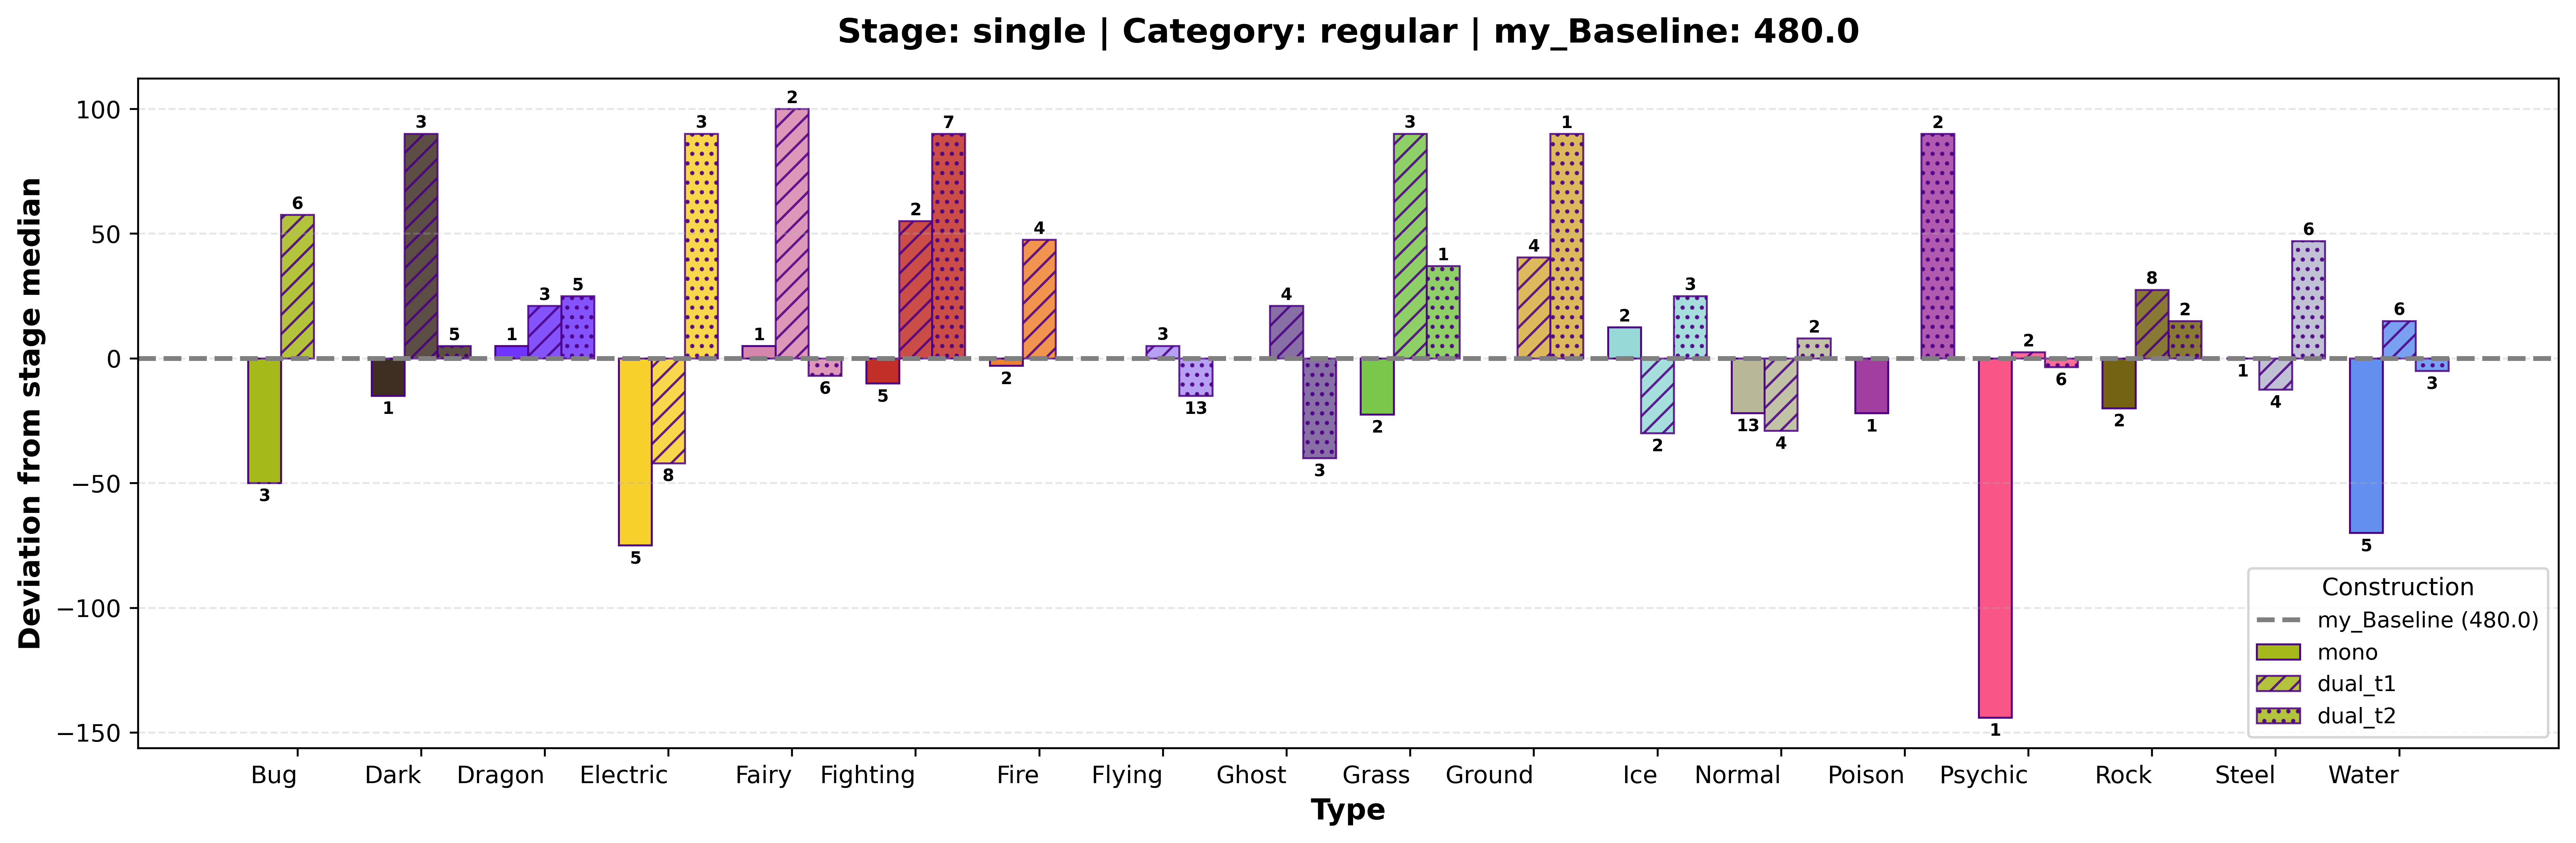
\includegraphics[width=\linewidth]{../plots/type_dev_single.png}
        \caption{Type deviations Single}
    \end{subfigure}
\end{figure}

\paragraph{Insights}
\begin{itemize}
    \item \textbf{Bug type:} Major negative deviation as primary/mono-type in finals/singles.
    \item \textbf{Normal type:} Negative except as secondary in singles (positive boost).
    \item \textbf{Dragon:} Consistently boosts BST regardless of position.
    \item \textbf{Fire/Water:} Strong in specific stages (S2c2/S3c3).
    \item \textbf{Missing combos:} No mono-Bug F3; no mono-Flying (non-legendary).
\end{itemize}

\subsection{Dual-Type Order Effects (\(\geq 3\) Pokémon per combo)}

\begin{figure}[H]
    \centering
    \begin{subfigure}{0.32\textwidth}
        \centering
        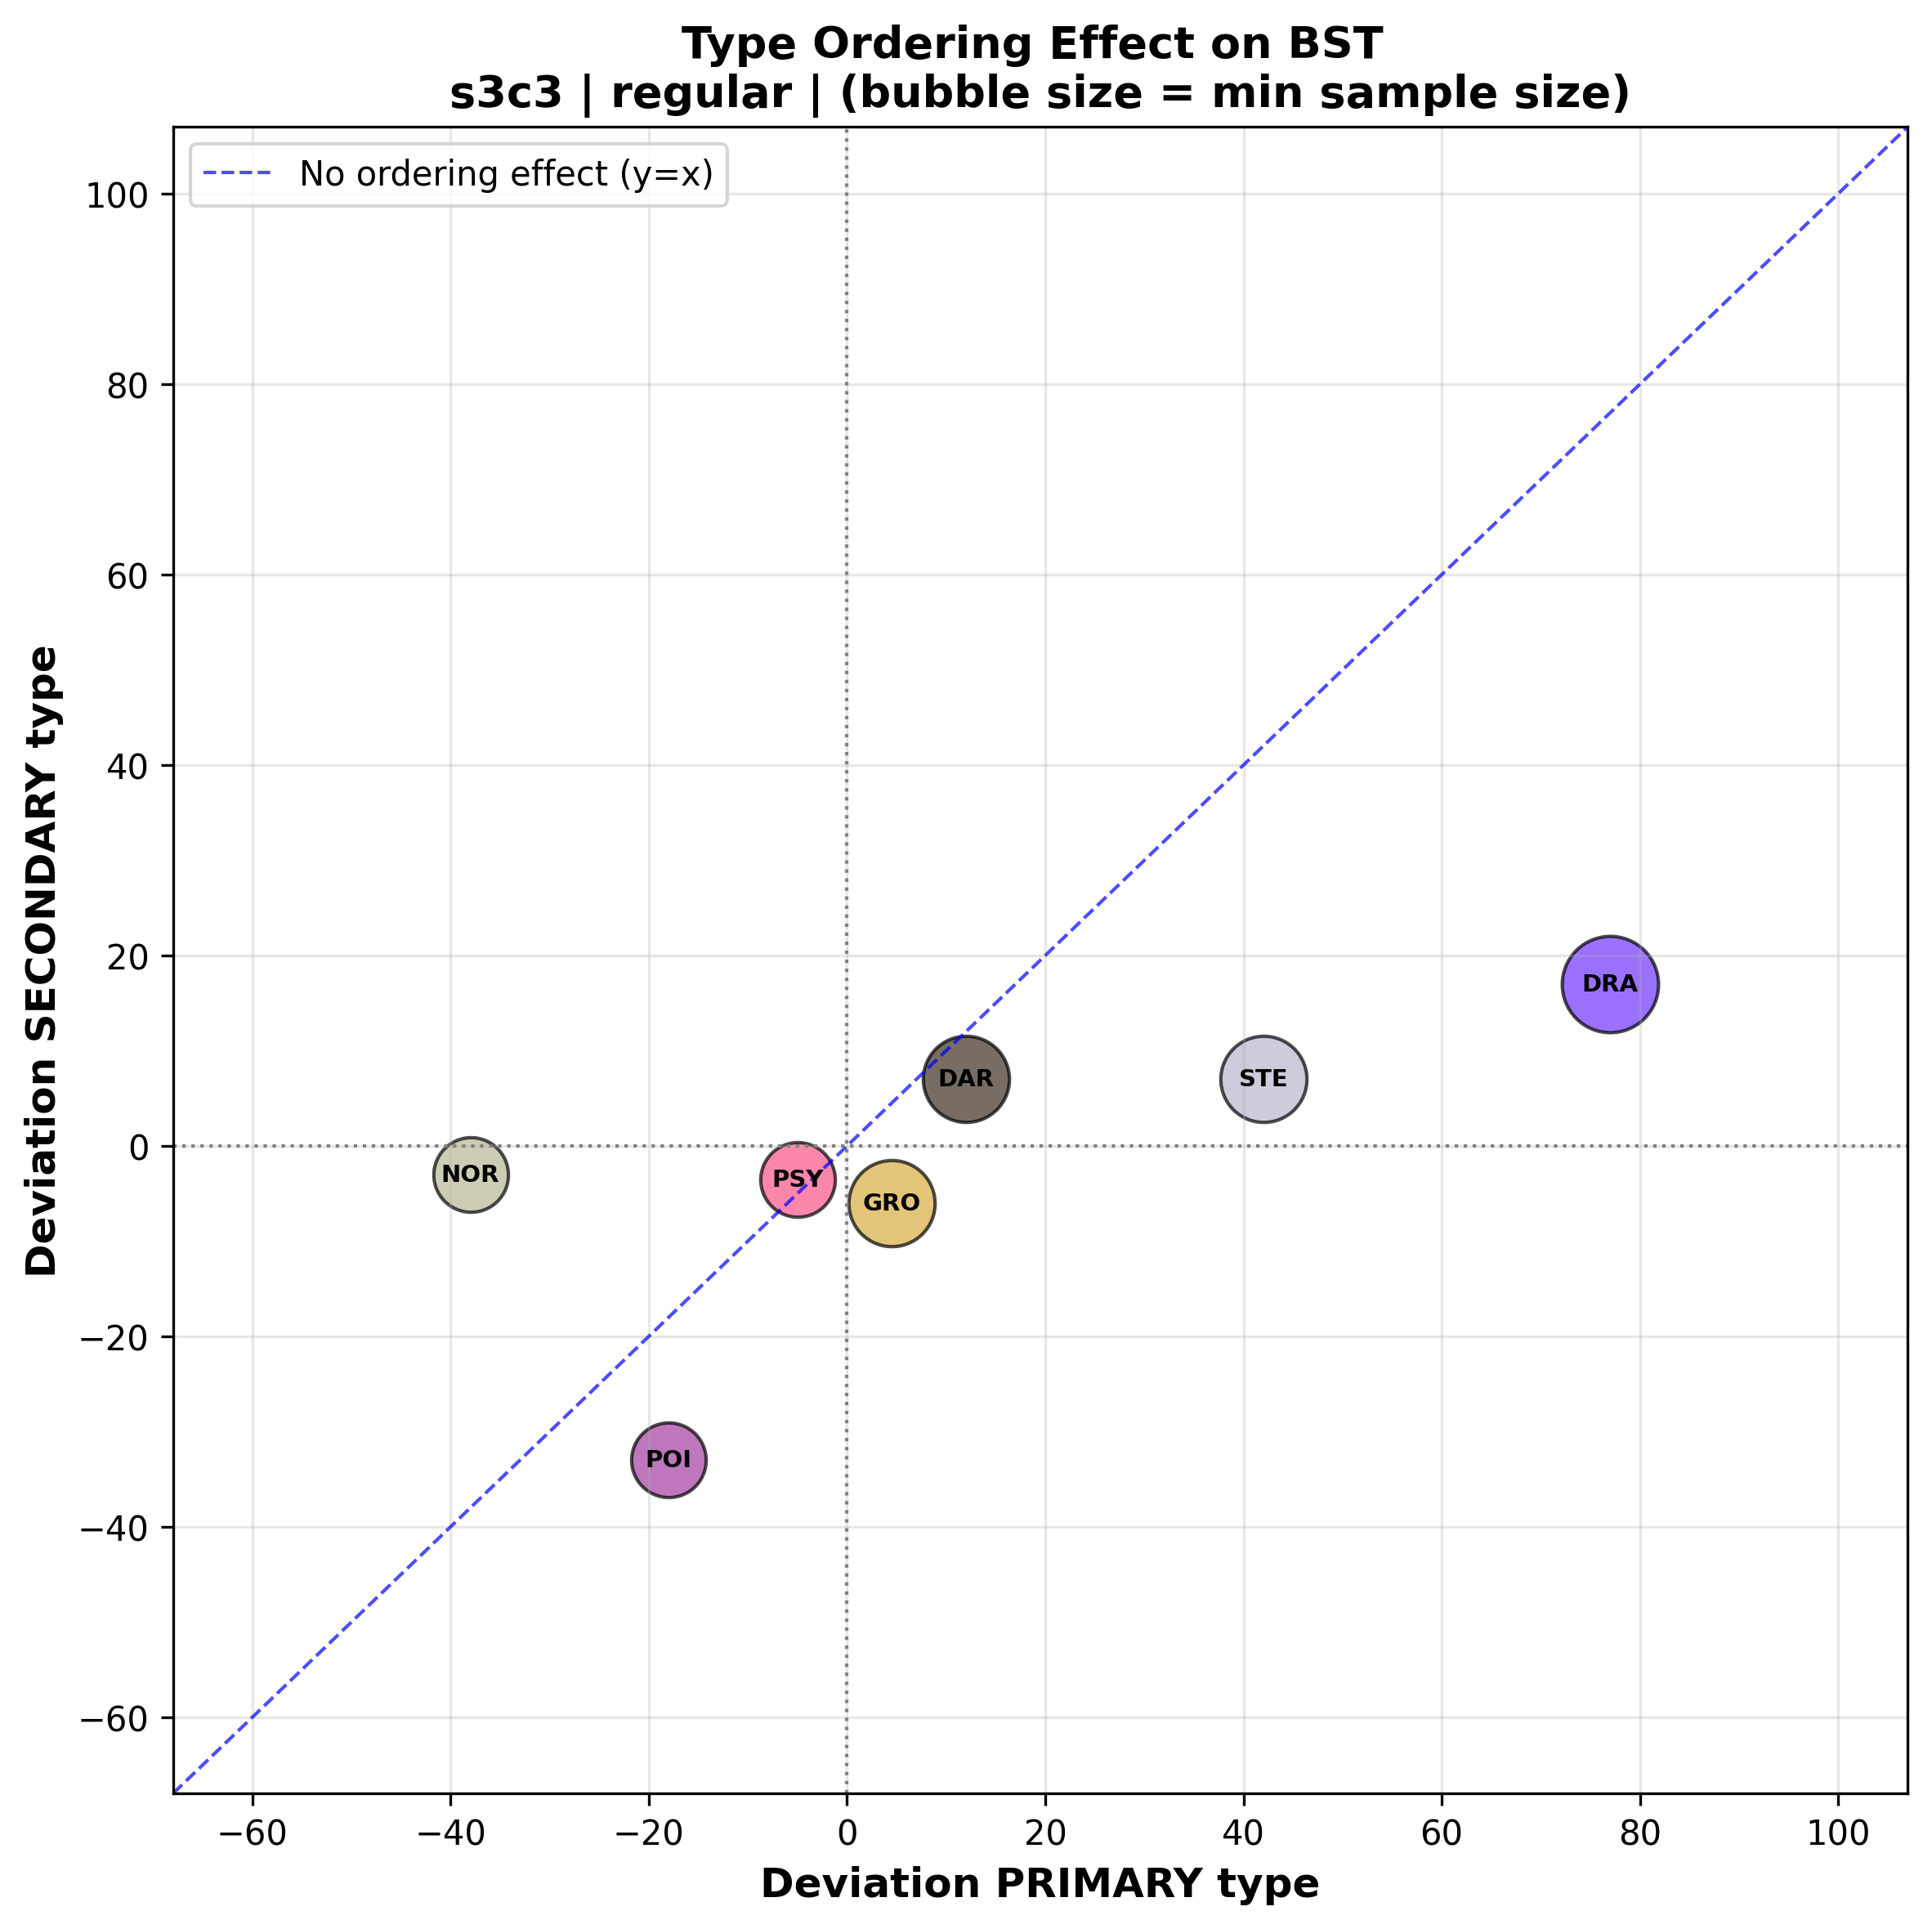
\includegraphics[width=\linewidth]{../plots/type_order_s3c3.png}
        \caption{Type order S3C3}
    \end{subfigure}
    \hfill
    \begin{subfigure}{0.32\textwidth}
        \centering
        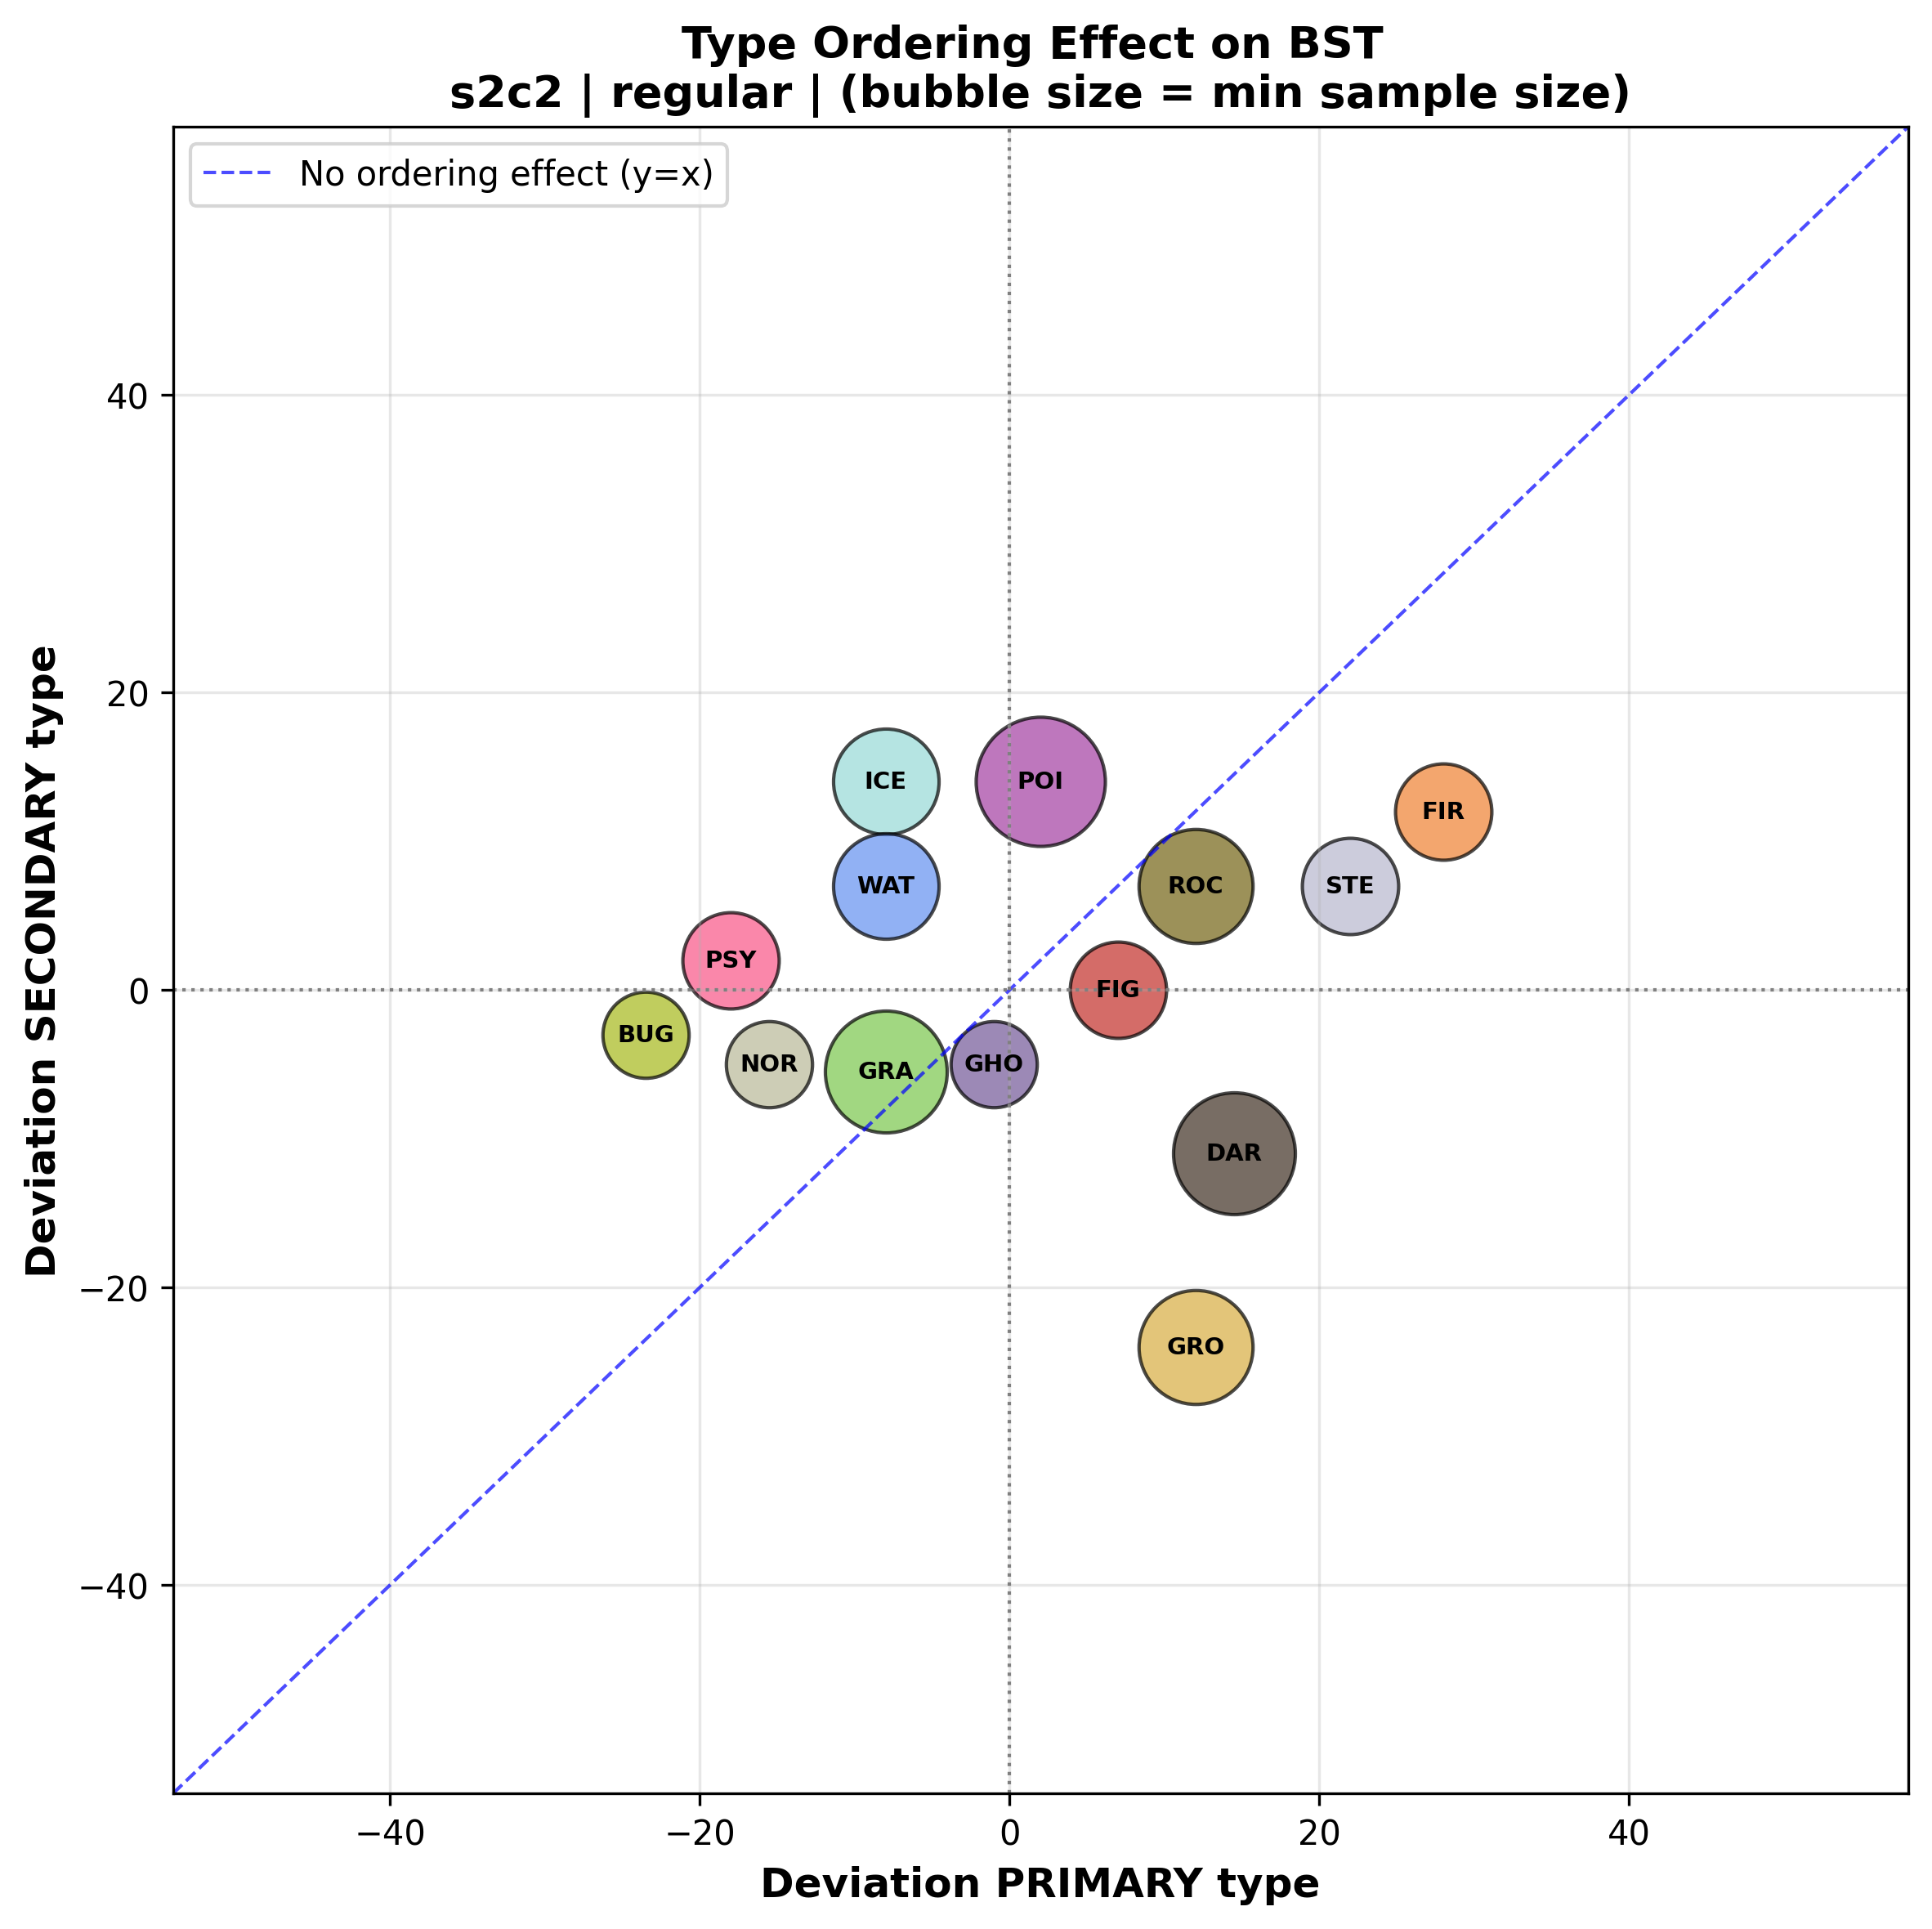
\includegraphics[width=\linewidth]{../plots/type_order_s2c2.png}
        \caption{Type order S2C2}
    \end{subfigure}
    \hfill
    \begin{subfigure}{0.32\textwidth}
        \centering
        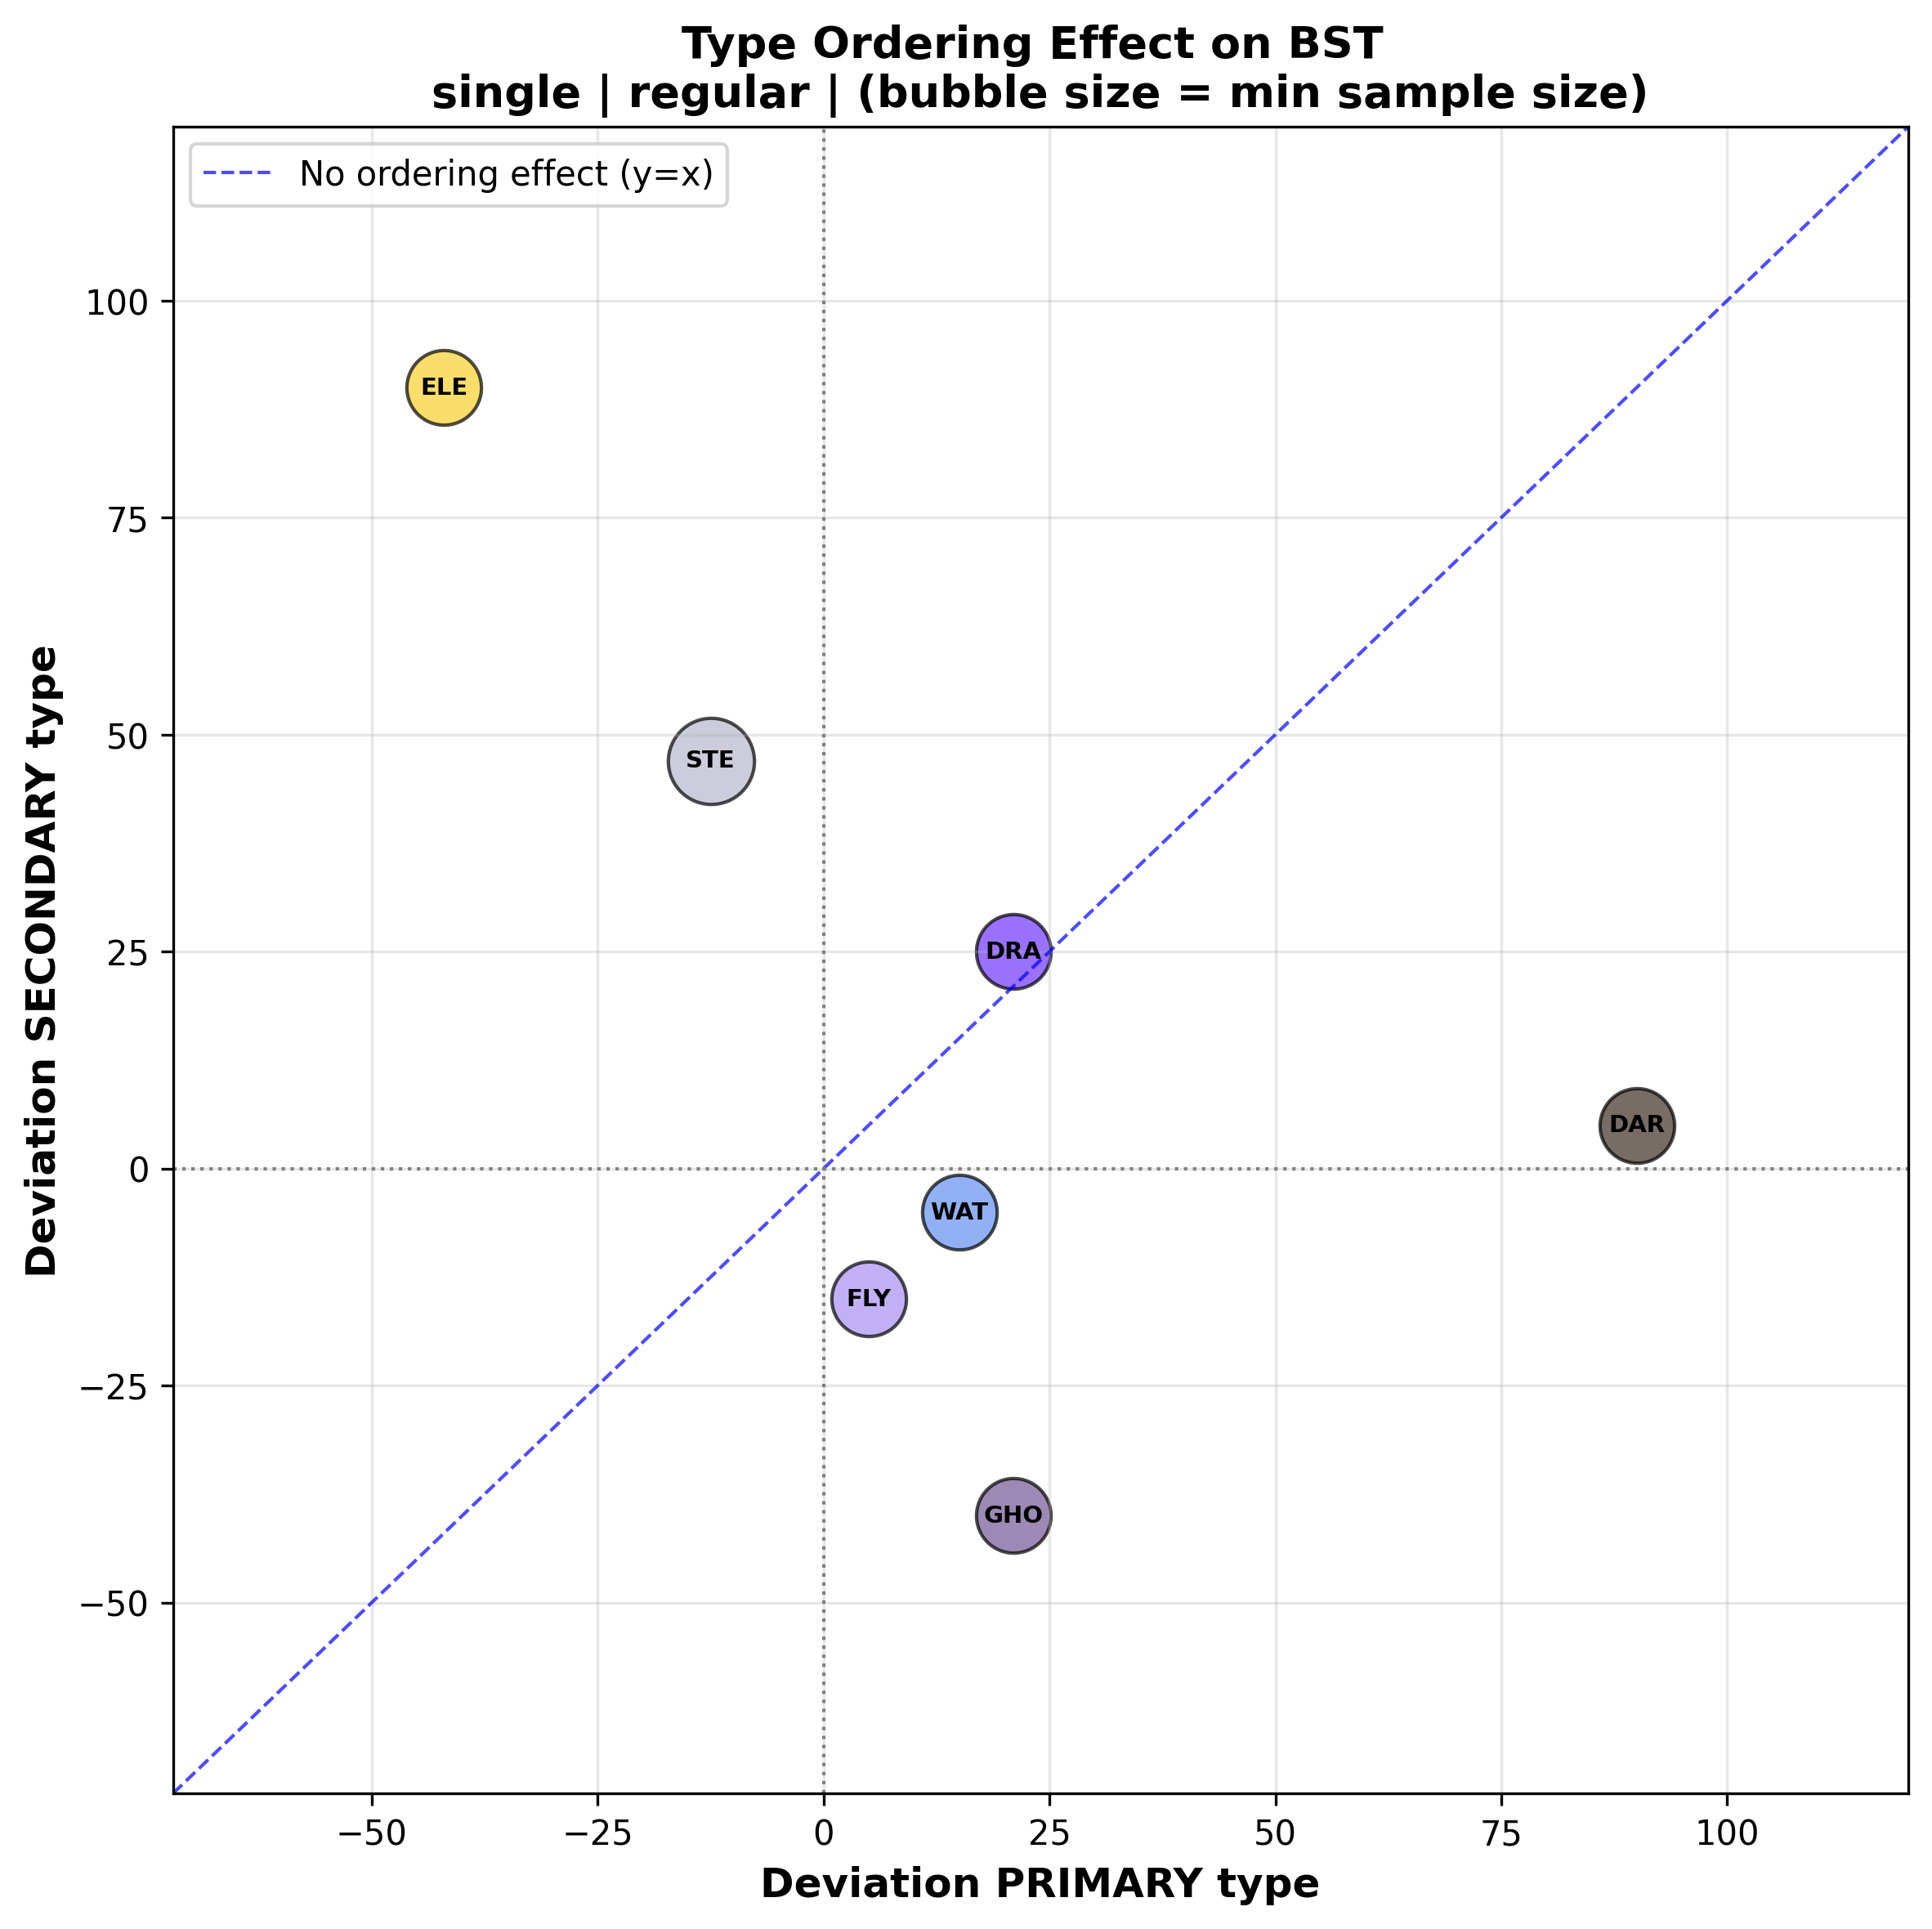
\includegraphics[width=\linewidth]{../plots/type_order_single.png}
        \caption{Type order Single}
    \end{subfigure}
\end{figure}

\paragraph{Findings}
\begin{itemize}
    \item Type ordering creates measurable BST differences in dual-types.
    \item Restricting to higher counts (>3 pairs) could reveal stronger patterns.
    \item \textbf{Game Freak experimentation potential} for Gen 10 type combos.
\end{itemize}

\section{Next Steps}

\textit{Work in progress---stay tuned for model results!}

\end{document}
